\documentclass[a4paper]{report}

% Use swiss german letters
\usepackage[utf8]{inputenc}

% Language: german
\usepackage[ngerman]{babel}

% Fancy Figures
\usepackage{graphicx}

% Subfigures
\usepackage{subcaption}

% Use Times
\usepackage{mathptmx}

% Display the Bibliography in the TOC
\usepackage{tocbibind}

% Better lists
\usepackage{enumitem}

% We want SI units!!!
\usepackage{siunitx}

% Formeln
\usepackage{amsfonts}

% Formeln
\usepackage{amsmath}

% Definierte Spaltenbreiten bei Tabellen
\usepackage{array}

% Use biblatex
\usepackage[style=apa,backend=biber,citestyle=authoryear]{biblatex}

% Footnote glue to bottom
\usepackage[bottom]{footmisc}

% Make references hyperlinks
\usepackage[hidelinks]{hyperref}

% To be able to use multiple columns
\usepackage{multicol}

% Tell BibLatex to use the ngerman language mapping
\DeclareLanguageMapping{ngerman}{ngerman-apa}

% Define the bibliography file
\addbibresource{bibliography.bib}

% To let LaTeX handle "
\usepackage[autostyle=true, german=quotes]{csquotes}

% Rename the Abstract to Management Summary
\addto\captionsngerman{\renewcommand{\abstractname}{Management Summary}}

% Titlepage
\newcommand*{\titleAP}{\begingroup % Create the command for including the title page in the document
	\centering
	\vspace*{\baselineskip} % Whitespace at the top of the page

	{Basil Bachmann, Pascal Baumann, David Craven, Victor Guntern, Markus Kempf, Eve Meier, Jan Odermatt, Simon Rohrer}\\[0.167\textheight] % Author name

	{\Huge\bfseries Projektdokumentation PREN Gruppe03}\\[\baselineskip]

	%TODO review subtitle
	{\Large \textit{Autonome Laufkatze}}\\
	\today

	\vspace*{3\baselineskip} % Whitespace at the bottom of the page
	\endgroup}

% Define the path were images are found
\graphicspath{{./img/}}

\begin{document}
\pagenumbering{gobble}

\titleAP

\newpage

\chapter*{Redlichkeitserklärung}
Hiermit erklären wir, dass wir die vorliegende Arbeit selbständig angefertigt haben und keine anderen als die angegebenen Hilfsmittel verwendet wurden. Sämtliche verwendeten Textauschnitte, Zitate oder Inhalte anderer Verfasser wurden ausdrücklich als solche gekennzeichnet.

\vspace{1.5em}

\noindent
Horw, \today

\vspace{2em}

\noindent
\begin{tabular}{lp{0.7\textwidth}}
	Basil Bachmann & \\[1em]
	\cline{2-2}
	Pascal Baumann &  \\[1em]
	\cline{2-2}
	David Craven & \\[1em]
	\cline{2-2}
	Victor Guntern & \\[1em]
	\cline{2-2}
	Markus Kempf & \\[1em]
	\cline{2-2}
	Eve Meier & \\[1em]
	\cline{2-2}
	Jan Odermatt & \\[1em]
	\cline{2-2}
	Simon Rohrer &  \\[1em]
	\cline{2-2}
\end{tabular}

\newpage

\pagenumbering{roman}
\begin{abstract}
	Hier würde man das Abstract oder Management Summary schreiben.
\end{abstract}

\chapter*{Versionierung}
\vspace{2em}

\noindent
\begin{tabular}{|c|p{0.7\textwidth}|}
	\hline
	\textbf{Versionsnummer} & \textbf{Beschreibung}\\
	\hline
	1.0 & Meileinstein 1 \\
	\hline
\end{tabular}

\tableofcontents

\newpage

\pagenumbering{arabic}

\chapter{Einleitung}
\label{ch:Intro}

Dieses Dokument beschreibt den Entwicklungsprozess einer autonomen Laufkatze. Dabei handelt es sich um ein interdiszpilinäres Projekt, welches über zwei Semester an der Hochschule Luzern absolviert wurde. In diesem Projekt musste mit einem begrenzten Budget gearbeitet und vielseitige Herausforderungen bewältigt werden.

In einer ersten Phase wurden vor allem Arbeitsprozesse ausgearbeitet, Recherchen betrieben und Konzepte entwickelt. Den schon frühen Entscheid mit \LaTeX die Dokumentation zu gestalten schien zuerst gewagt, die einzelnen Teammitglieder lernten jedoch schnell mit diesem neuen Werkzeug zu arbeiten.

\chapter{Projektorganisation}

\section{Teamübersicht}

\begin{tabular}{|p{0.3\textwidth}|p{0.3\textwidth}|}
	\hline
	\textbf{Name} & \textbf{Studium} \\
	\hline
	Basil Bachmann & Maschinenbau \\
	\hline
	Pascal Baumann & Informatik \\
	\hline
	David Craven & Elektrotechnik \\
	\hline
	Victor Guntern & Maschinenbau \\
	\hline
	Markus Kempf & Maschinenbau \\
	\hline
	Eve Meier & Informatik \\
	\hline
	Jan Odermatt & Elektrotechnik \\
	\hline
	Simon Rohrer & Maschinenbau \\
	\hline
\end{tabular}

\section{Projektrollen}

\begin{tabular}{|p{0.3\textwidth}|p{0.5\textwidth}|p{0.2\textwidth}|}
	\hline
	\textbf{Rolle} & \textbf{Aufgaben} & \textbf{Teammitglied} \\
	\hline
	Projektleiter & Gesamtübersicht des Projektes halten  & Eve \\
	& Überprüfen ob Vorgaben eingehalten werden & \\
	& Teammeetings organisieren & \\
	& Informationsaustausch sicherstellen & \\
	& Kostenverwaltung & \\
	\hline
	Projektplaner & Aktualisieren des Terminplanes & Markus\\
	& Rahmenplanung und Überblick über Einhaltung Meilensteine& \\
	& Pflege Taskboard & \\
	\hline
	Verantwortlicher Dokumentation& Zusammenstellen des Abgabedokuments für Meilensteine & Pascal \\
	& Unterstützung und Pflege LaTeX &  \\
	\hline
	Protokollführer & Protokolle führen & Simon \\
	& Alte Protokolle abnehmen lassen & \\
	\hline
	Fachverantwortliche & Projektstand und Feedback & I Pascal \\
	& Ansprechperson bei Fragen & ET Jan\\
	& Aktualisierung Risikomanagement & M Markus\\
	& Koordination Versuche und Recherche & \\
	\hline
\end{tabular}

\section{Tools}
\begin{tabular}{|p{0.4\textwidth}|p{0.6\textwidth}|}
	\hline
	\textbf{Aufgabe} & \textbf{Hilfsmittel} \\
	\hline
	Dokumente und Dokumentation & LaTeX / MiKTeX / GitHub \\
	\hline
	Quellen & Mendeley \\
	\hline
	Dateiablage für Teamaustausch & Dropbox \\
	\hline
	Dateiablage für Abgabe & Ilias \\
	\hline
	Projekt- und Budgetplan & MS Excel 2016 \\
	\hline
	Kommunikation Team & WhatsApp Gruppe oder über die HSLU Mailadresse\\
	\hline
	Aufgabenverwaltung & SCRUM-angelehntes Board, physisch, Teaminsel\\
	\hline
\end{tabular}

\section{Wochenplan}
\begin{tabular}{|p{0.2\textwidth}|p{0.8\textwidth}|}
	\hline
	\textbf{Tag} & \textbf{Beschreibung} \\
	\hline
	DO 08:30 & Alle Mitglieder sind in der Teaminsel \\
	\hline
	DO 08:30-09:00 & Besprechung Team-intern erledigte Aufgaben \\
	& Fragen, weiteres Vorgehen \\
	\hline
	DO 09:00-10:00 & Arbeiten im Team od. selbständig \\
	\hline
	DO 10:00-10:20 & Pause \\
	\hline
	DO 10:20-12:00 & Arbeiten im Team od. selbstständig \\
	\hline
	FR 08:30 & Alle Mitglieder sind in der Teaminsel \\
	\hline
	FR 08:30-09:00 & Besprechung Team-intern, Vorbereitung Meeting mit Dozent \\
	\hline
	FR 09:00-09:30& Besprechung mit Dozent \\
	\hline
	FR 09:30-10:00 & Arbeiten im Team od. selbstständig \\
	\hline
	FR 10:00-10:20 & Pause \\
	\hline
	FR 10:20-11:00 & Arbeiten im Team od. selbstständig \\
	\hline
	FR 11:00-11:30 & Kurzbesprechung, Taskboard aktualisieren \\
	\hline
	FR 11:30-12:00 & Arbeiten im Team oder selbstständig (freiwillig)\\
	\hline
\end{tabular}

\section{Projektplan}

An dieser Stelle ist der Projektplan grob umrissen, den Detaillierten finden Sie im Anhang.

\begin{figure}[h!]
	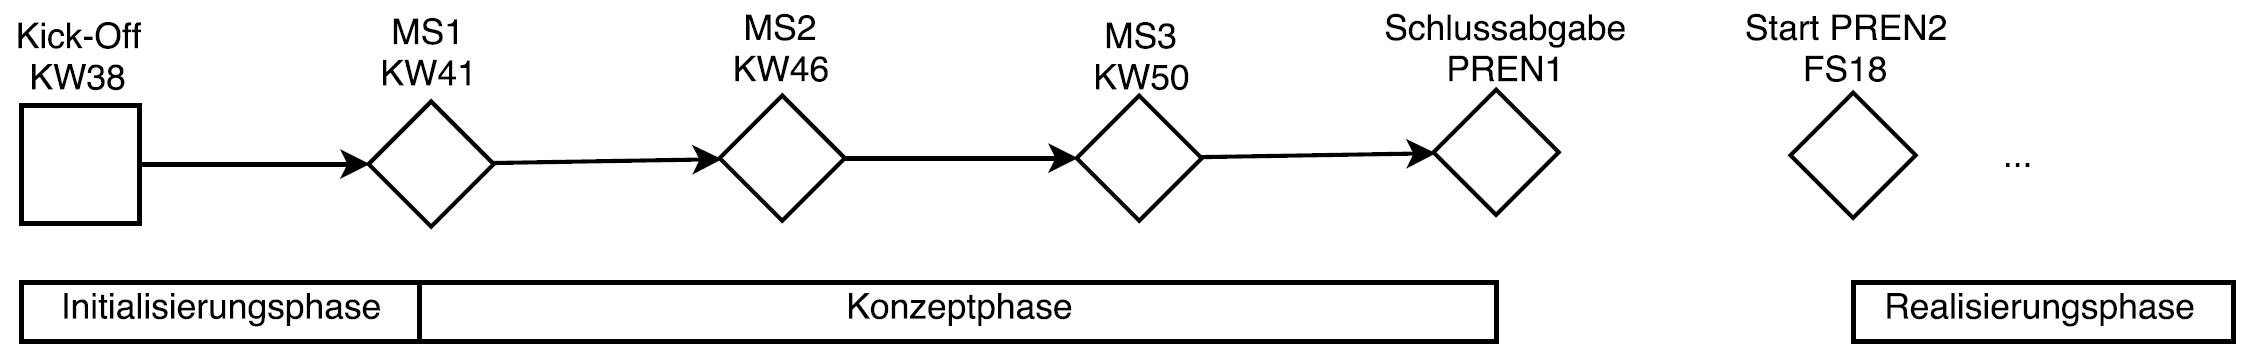
\includegraphics[width=\linewidth,keepaspectratio]{Rahmenplan}
	\caption{Grober Projektplan}
	\label{fig:GrobProjekt}
\end{figure}

\vspace{1em}
\noindent
\begin{tabular}{|p{0.2\textwidth}|p{0.2\textwidth}|p{0.55\textwidth}|}
	\hline
	\textbf{Meileinstein} & \textbf{Termin} & \textbf{Beschreibung} \\
	\hline
	Start & 21.09.2017 & Input 1 mit Einfürung \\
	\hline
	Meilenstein 1 & 13.10.2017 12:00 Uhr & Projektorganisation, Technologierecherche, Anforderungsliste \\
	\hline
	Meilenstein 2 & 10.11.2017 12:00 Uhr & Risikomanagement, Evaluation der Lösungsprinzipien und Auswahl der optimalen Lösungskombination(en) \\
	\hline
	Meilenstein 3 & 15.12.2017 12:00 Uhr & Freigabe des Gesamtkonzepts, Dokumentation zu 80\% fertig gestellt. \\
	\hline
	Schlussabgabe PREN1 &12.01.2018 & Schlussabgabe Dokumentation zu 100\% fertig \\
	\hline
\end{tabular}

\section{Budgetplan}
Für den Bau der Teilfunktionsmuster in PREN1 dürfen maximal CHF 200.- ausgegeben werden. Dieser Teil dient daher vor allem der Kostenverfolgung, damit das Budget nicht überzogen wird.

\vspace{1em}
\noindent
\begin{tabular}{|p{0.225\textwidth}|p{0.225\textwidth}|p{0.225\textwidth}|p{0.225\textwidth}|}
	\hline
	\textbf{Artikel} & \textbf{Anzahl} & \textbf{Preis/Stk. CHF} & \textbf{Total CHF} \\
	\hline
	Artikel 1 & 2 & 11.50 & 23 \\
	\hline
	\textbf{Total} & & & 23 \\
	\hline
\end{tabular}


\chapter{Anforderungen}
\section{Kurzbeschrieb Anforderungen}
Das Gerät muss sich autonom an einem ansteigenden Drahtseil fortbewegen können. Eine Last muss an einem bestimmten Ort aufgehoben werden, ohne Berührung über Hindernisse transportiert, und danach möglichst exakt auf einer Zielplatte abgesetzt werden. Nach dem Absetzen der Last muss das Gerät den Zielraum erreichen und den Masten berühren. Die Zielplatte muss das Gerät selbstständig erkennen können. Das Gerät darf nur die Last, das Drahtseil und den zweiten Masten berühren. Nach Aufnahme der Last muss die aktuelle Position der Last in x-, und z-Richtung in Echtzeit dargestellt werden. Das Gerät muss innerhalb von zwei Minuten startbereit sein. Die Zeit um den Zielraum zu erreichen liegt bei maximal vier Minuten. In der Abbildung \ref{fig:Funktionsskizze} sehen Sie dies bildlich.


\begin{figure}[h!]
	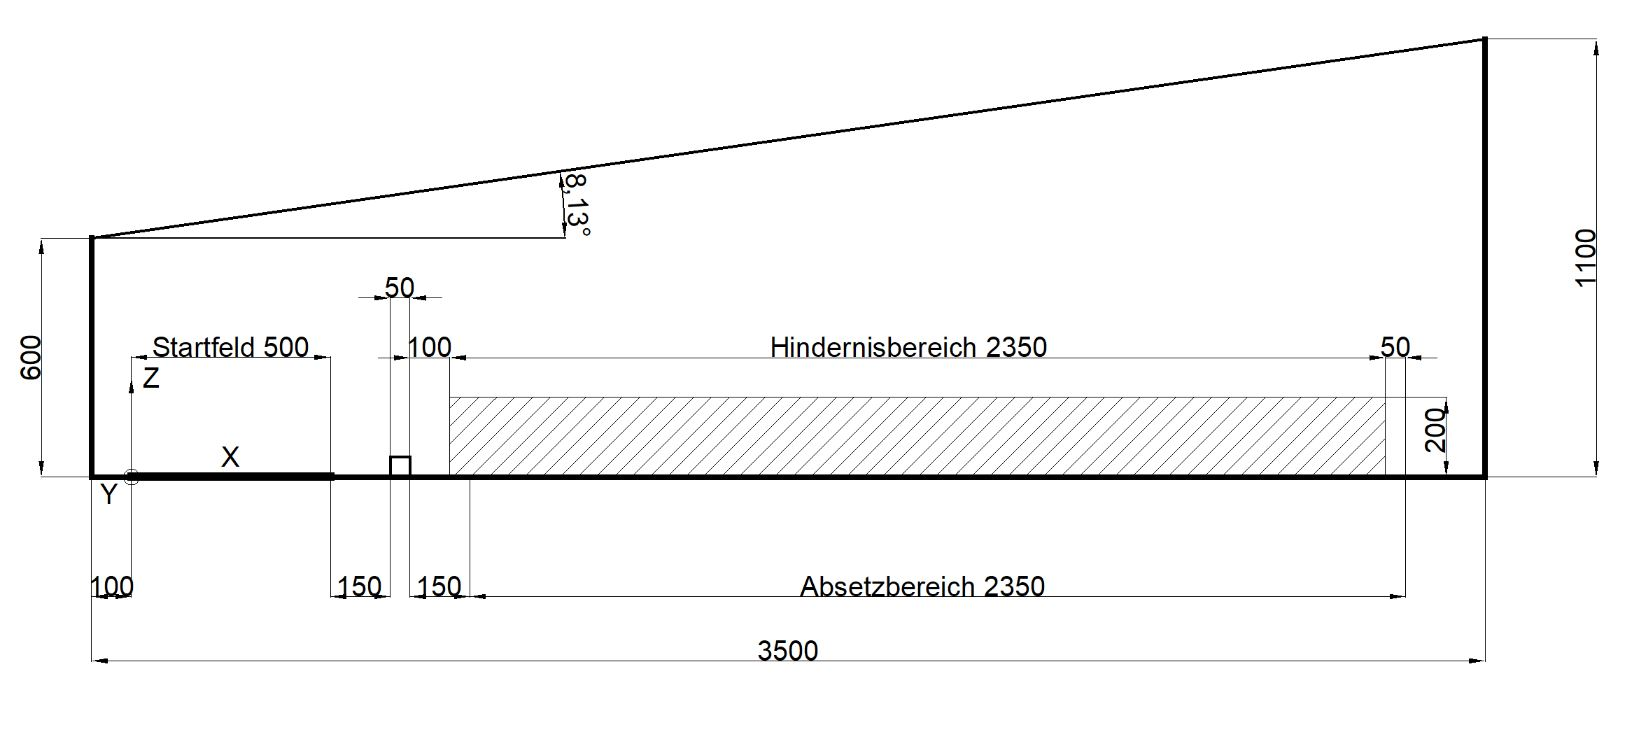
\includegraphics[keepaspectratio,width=\textwidth]{PrenFunktionsskizze}
	\caption{Skizze des Versuchsaufbaus}
	\label{fig:Funktionsskizze}
\end{figure}

\section{Projektanforderungen}
\begin{tabular}{|p{.05\textwidth}|p{0.07\textwidth}|p{0.3\textwidth}|p{0.55\textwidth}|}
	\hline
	\textbf{Nr.} & \textbf{FMW\footnotemark} & \textbf{Bezeichnung} & \textbf{Beschreibung} \\
	\hline
	1.1 & F & Projektabgabe & Dezember 2017 \\
	\hline
	1.2 & F & Eigenleistung & Systemkomponenten können zugekauft werden \\
	\hline
	1.3 & F & Interdisziplinarität & Disziplinen / Abteilungen arbeiten zusammen \\
	\hline
	1.4 & W & Lieferantenwahl & Für Sammelbestellungen gem. Kapitel 4.5 der Aufgabenstellung. Wird Material vom Team selbst gekauft, können die Kosten zurückgefordert werden \\
	\hline
	1.5 & M & Budget f. PREN & max. 500.- CHF \\
	\hline
	1.6 & M & Teilbudget PREN1 & max. 200.- CHF \\
	\hline
	1.7 & M & 3D-Drucker Laufzeit & max. 25h \\
	\hline
	1.8 & M & Lasergerät Laufzeit & max. 1h \\
	\hline
	1.9 & M & Stunden ET-Werkstattpersonal & max. 10h \\
	\hline
	1.10 & M & Stunden M-Werkstattpersonal & max. 10h \\
	\hline
	1.11 & F & "Gesponsorte"\ Komponenten & Werden mit einem realistischen Preis in die Kostenrechnung einbezogen \\
	\hline
\end{tabular}
\footnotetext{F: Festanforderung M: Mindestanforderung W: Wunschanforderung }

\section{Plattform}
\begin{tabular}{|p{.05\textwidth}|p{0.07\textwidth}|p{0.3\textwidth}|p{0.55\textwidth}|}
	\hline
	\textbf{Nr.} & \textbf{FMW\footnotemark} & \textbf{Bezeichnung} & \textbf{Beschreibung} \\
	\hline
	2.1 & F & Gesamtlänge & 350 $\pm$ 2cm \\
	\hline
	2.2 & F & Masten Abstand & Abstand zwischen den Masten 350cm $\pm$ 2cm \\
	\hline
	2.3 & F & Masten Masse & 8cm Front, 6cm Tiefe \\
	\hline
	2.4 & F & Drahtseil & Verzinkter Stahl, Durchmesser 3mm \\
	\hline
	2.5 & F & Seilspannung & Via Umlenkrollen durch ein Gewicht mit einer Masse von 15kg \\
	\hline
	2.6 & F & Winkel des Seiles & TODO \\
	\hline
	2.7 & F & Grundplatte & Spanplatte roh oder grau gestrichen.\\
	& & & Mit Farbresten / vorstehenden Schrauben und Nahtstellen ist zu rechnen \\
	\hline
	2.8 & F & Startfeld & 50cm $\pm$ 2cm, Quadratisch \\
	\hline
	2.9 & F & Zielplatte & TODO Gesamtmass? \\
	\hline
	2.10 & F & Zielplatte Aussehen & TODO Wie viele konzentrische Bereiche?\\
	& & & Der innerste, helle Bereich ist quadratisch und hat eine Seitenlänge von 6cm $\pm$ 2mm. \\
	& & & Jeder daran anschliessende konzentrische Bereich hat eine Breite von 2.5cm $\pm$ 2mm. \\
	& & & Die Bereiche sind abwechslungsweise hell und dunkel \\
	\hline
	2.11 & F & Zielplatte Position & Der Absetzbereich verläuft unterhalb des Seiles und ist 2cm breit.\\
	& & & Die Zielplatte kann bis zum Startsignal verschoben werden.\\
	& & & Befindet sich aber immer im Absetzbereich (siehe Abbildung 1 der Aufgabenstellung) \\
	\hline
	2.12 & F & Start- und Zielplatte & TODO Matt? Glänzend? \\
	\hline
	2.13 & F & Hindernisse & Auf der gesamten Plattform können Hindernisse stehen.\\
	& & & Im Umkreis von mindestens 10cm um die Startposition des Ladegutes und um die Zielplatte herum sind keine Hindernisse \\
	\hline
	2.14 & M & Hindernisse Höhe & Die Hindernisse haben eine maximale Höhe von 20cm. \\
	\hline
\end{tabular}
\footnotetext{F: Festanforderung M: Mindestanforderung W: Wunschanforderung }

\section{Laufkatze}
\begin{tabular}{|p{.05\textwidth}|p{0.07\textwidth}|p{0.3\textwidth}|p{0.55\textwidth}|}
	\hline
	\textbf{Nr.} & \textbf{FMW\footnotemark} & \textbf{Bezeichnung} & \textbf{Beschreibung} \\
	\hline
	3.1 & F & Steuerung & Autonom \\
	\hline
	3.2 & M & Inbetriebnahme & Darf max. 2min dauern \\
	\hline
	3.3 & M & Startsignal & Darf per Kopfdruck gesendet werden \\
	\hline
	3.4 & M & Geschwindigkeit & Um die Aufgabe zu bewältigen steht der Laufkatze\\
	& & & ein Zeitfensters von 4min zur Verfügung. \\
	\hline
	3.5 & M & Aussendimensionen & Die Laufkatze darf in ihrer Projektion das Startfeld nicht überschreiten. 50cm $\pm$ 2cm x 50cm $\pm$ 2cm \\
	\hline
	3.6 & F & Bauart & Sämtliche Sensorik muss auf dem Gerät selbst montiert sein. \\
	\hline
	3.7 & F & Fahrweise & Das Gerät darf nur das Drahtseil und den zweiten Masten berühren.\\
	& & & Die gesamte Plattform, insbesondere Drahtseil, die Last und die Zielplatte dürfen nicht beschädigt oder sonst irgendwie verändert werden.\\
	& & & Es ist beispielsweise nicht erlaubt, Navigationshilfen anzubringen. \\
	\hline
	3.8 & F & Ladegut & Das Gerät muss ein Ladegut transportieren können. \\
	\hline
	3.9 & F & Zielerkennung & Das Erkennen der Zielplatte muss selbstständig erfolgen\\
	\hline
\end{tabular}
\footnotetext{F: Festanforderung M: Mindestanforderung W: Wunschanforderung }

\section{Ladegut}
\label{sec:AnfLadegut}
\begin{tabular}{|p{.05\textwidth}|p{0.07\textwidth}|p{0.3\textwidth}|p{0.55\textwidth}|}
	\hline
	\textbf{Nr.} & \textbf{FMW\footnotemark} & \textbf{Bezeichnung} & \textbf{Beschreibung} \\
	\hline
	4.1 & F & Material & Holz \\
	\hline
	4.2 & F &  Dimensionen & Seitenlänge 5cm $\pm$ 0.5cm \\
	\hline
	4.3 & M & Gewicht & 50-90g, siehe Sektion \ref{sec:RechKlotzMasse} \\
	\hline
	4.4 & F & Aufnahme & Metallischer, magnetischer Hacken oben in der Mitte des Würfels.\\
	& & & Innendurchmesser des Hakens ist 1.3cm $\pm$ 0.1mm\\
	\hline
	4.5 & F & Hindernisse & Das Ladegut darf Hindernisse nicht berühren. \\
	\hline
	4.6 & F & Position & Die Position des Ladegutes muss in Echtzeit angezeigt werden, dass der Schiedsrichter jederzeit die angezeigten Werte gut erkennen kann.\\
	& & & TODO auf Gerät od. Extern? \\
	\hline
	4.7 & F & Positionsbestimmung & Die Mitte des Bodens des Ladegutes wird verwendet.\\
	& & & Die Position muss in x- und z-Richtung bestimmt werden (siehe Skizze Anforderungen).\\
	& & & Der Nullpunkt des zu verwendenden Koordinatensystems ist in Abbildung 1 der Aufgabenstellung definiert. \\
	\hline
	4.8 & F & Absetzen & Das Ladegut muss innerhalb des Zielbereiches automatisch abgesetzt werden. \\
	\hline
	4.9 & F & Zielbereich & Der Zielbereich muss automatisch erkennt werden\\
	\hline
\end{tabular}
\footnotetext{F: Festanforderung M: Mindestanforderung W: Wunschanforderung }

\section{Umfeld}
\begin{tabular}{|p{.05\textwidth}|p{0.07\textwidth}|p{0.3\textwidth}|p{0.55\textwidth}|}
	\hline
	\textbf{Nr.} & \textbf{FMW\footnotemark} & \textbf{Bezeichnung} & \textbf{Beschreibung} \\
	\hline
	5.1 & M & Licht & Scheinwerfer welche auf die Wettbewerbsplattformen gerichtet sind, werden dazu führen, dass wir mit einer hohen Helligkeit arbeiten müssen \\
	\hline
	5.2 & M & Temperaturen & Bei Lagerung und Betrieb Zimmertemperatur 15-\SI{20}{\degreeCelsius}\\
	\hline
	5.3 & M & Kein Spritzwasser & Für Innenanwendung\\
	\hline
	5.4 & M & Keine Hochspannung & Normale Netzspannung\\
	\hline
\end{tabular}
\footnotetext{F: Festanforderung M: Mindestanforderung W: Wunschanforderung }

\chapter{Risikomanagement}
In diesem Kapitel werden mögliche Risiken während des Projektverlaufes aufgelistet. Dabei werden Projektrisiken nummeriert. Ihre Eintrittswahrscheinlichkeit und ihr Schadensausmass wird eingeschätzt. Besteht ein grosses Risiko, werden zusätzlich Massnahmen definiert.

\section{Definitionen}

%TODO Stimmen dieses vertical Spacers noch?
\vspace{1em}
\noindent
Eintrittswahrscheinlichkeit:

%TODO Stimmen dieses vertical Spacers noch?
\vspace{1em}
\noindent
\begin{tabular}{|p{0.06\textwidth}|p{0.2\textwidth}|p{0.7\textwidth}|}
	\hline
	\textbf{Stufe} & \textbf{Bezeichnung} & \textbf{Beschreibung} \\
	\hline
	1 & unvorstellbar & Möglich aber eher unwahrscheinlich. Tritt nie oder einmal in 14 Wochen auf \\
	\hline
	2 & unwahrscheinlich & Kann in 14 Wochen 1-5 Mal eintreten\\
	\hline
	3 & vorstellbar & Kann in 14 Wochen 6-8 Mal eintreten \\
	\hline
	4 & wahrscheinlich & Kann in 14 Wochen bis zu 10 Mal eintreten \\
	\hline
	5 & häufig & Kann in 14 Wochen 14 Mal eintreten\\
	\hline
\end{tabular}

%TODO Stimmen dieses vertical Spacers noch?
\vspace{1em}
\noindent
Schadensausmass:

\vspace{1em}
\noindent
\begin{tabular}{|p{0.06\textwidth}|p{0.2\textwidth}|p{0.7\textwidth}|}
	\hline
	\textbf{Stufe} & \textbf{Bezeichnung} & \textbf{Beschreibung} \\
	\hline
	1 & unwesentlich & Die Aufgabenerfüllung wird höchstens geringfügig beeinträchtigt finanzieller Schaden ist im Rahmen des Projekts nicht beeinflussend. Personenschäden treten nicht auf \\
	\hline
	2 & geringfügig & Wahrnehmbare Gefährdung / Einfluss auf das Projekt. Personenschäden treten nicht auf \\
	\hline
	3 & mittelmässig & Wahrnehmbare Gefährdung / Einfluss auf das Projekt.Finanzieller Schaden strapaziert das Projektbudget
	Personenschäden treten nicht auf \\
	\hline
	4 & kritisch & Starke Gefährdung des Projekts. Finanzieller Schaden übersteigt das Projektbudget massiv. Personenschäden treten geringfügig auf \\
	\hline
	5 & katastrophal & Projektabbruch zur Folge. Finanzieller Schaden kann zum Projektstopp führen. Verletzung der Persönlichkeitsrechte
	\\
	\hline
\end{tabular}


\section{Risikokatalog}

Legende:
\begin{itemize}
	\item \textbf{S}chadensausmass bei Eintreffen des Risikos
	\item \textbf{W}ahrscheinlichkeit das Risiko eintrifft
	\item \textbf{K}ategorie: \textbf{T}echnisches oder \textbf{P}rojektbezogenes Risiko
	\item \textbf{A}uswirkung auf das Projekt. Produkt aus S und W
\end{itemize}

\vspace{1em}
\noindent
\begin{tabular}{|p{0.03\textwidth}|p{0.75\textwidth}|p{0.03\textwidth}|p{0.03\textwidth}|p{0.03\textwidth}||p{0.03\textwidth}|}
	\hline
	\textbf{Nr.} & \textbf{Beschreibung / Risiko} & \textbf{K} & \textbf{S} & \textbf{W} & \textbf{A} \\
	\hline
	1 & Datenverlust & P & 5 & 1 & 5\\
	\hline
	2 & Zerstörung elektronischer Komponenten durch ESD & T & 3 & 3 & 9 \\
	\hline
	3 & Störung der Steuerungskomponenten durch Elektromotoren & T & 3 & 2 & 6 \\
	\hline
	4 & Fortbewegungsschwierigkeiten des Gerätes & T & 5 & 2 & 10 \\
	\hline
	5 & Schwankungen des Gerätes & T & 2 & 3 & 6 \\
	\hline
	6 & Probleme beim Transport der Last & T & 4 & 2 & 8 \\
	\hline
	7 & Probleme Fertigung oder Beschaffung Komponenten & P & 2 & 3 & 6 \\
	\hline
	8 & Stop über Zielplatzform schlägt fehl & T & 4 & 2 & 8 \\
	\hline
	9 & Fehlkommunikation im Team & P & 3 & 3 & 9 \\
	\hline
	10 & Teammitglied fällt aus & P & 3 & 2 & 6 \\
	\hline
	11 & Verzug bei Erstellung von Dokumenten & P & 3 & 2 & 6 \\
	\hline
	12 & Gerät startet nicht & T & 5 & 1 & 5 \\
	\hline
\end{tabular}

\section{Risikobewertung}

\begin{figure}[h!]
	\centering
	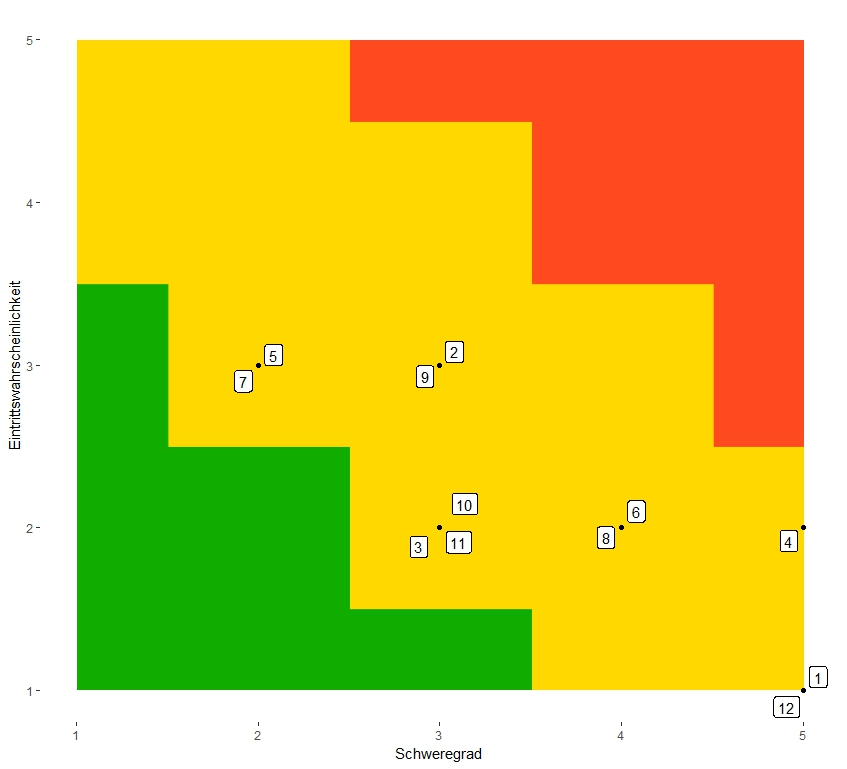
\includegraphics[width=.6\textwidth,keepaspectratio]{Risikomatrix}
	\caption{Die Risiken aus dem Risikokatalog graphisch dargestellt}
	\label{fig:Risikomatrix}
\end{figure}

\section{Massnahmen}
% TODO Stimmen diese vertikalen Spacers noch?
\vspace{1em}
\noindent
\begin{tabular}{|p{0.1\textwidth}|p{0.9\textwidth}|}
	\hline
	\textbf{Risiko Nr.} & \textbf{Massnahme} \\
	\hline
	1 & Es wird sowohl für Dokumentation und Programmcode mit GitHub als Versionskontrollsystem gearbeitet. Sonstige Daten befinden sich in der Dropbox. Dropbox wird als sicher eingestuft. \\
	\hline
	2 & Gesamtes Team ist im Umgang mit elektronischen Komponenten geschult. \\
	\hline
	3 & Magnetische Abschirmung des Elektromotors ist vorgesehen. Klare Aufteilung der Printplatte in Digital und Analog. \\
	\hline
	4 & Grösst mögliche Steigung des Seiles wird miteinbezogen. Laufkatze wird gegen rutschen und abstürzen gesichert. Akkuleistung wird genügend gross gewählt. \\
	\hline
	5 & Stabilisierung des Gerätes durch Gewicht oder Dämpfer. \\
	\hline
	6 & Erkennen, greifen und absetzen der Last muss durch Tests in 9 von 10 Mal funktionieren. \\
	\hline
	7 & Aufträge werden frühzeitig in Auftrag gegeben. Vor Auftragserteilung und Bestellung werden diese durch mindestens zwei Personen Überprüft.\\
	\hline
	8 & Zielerkennung wird unter verschiedenen Bedingungen (zum Beispiel Lichteinflüssen) getestet und muss in 9 von 10 Mal funktionieren. Laufkatze soll vor- und rückwärts fahren können. \\
	\hline
	9 & Bei Unklarheiten und Unwohlsein wird von jedem Teammitglied erwartet, dass er sich selbst meldet. Zur Veranschaulichung technischer Aspekte wird mit Skizzen gearbeitet. \\
	\hline
	10 & Aktueller Stand ist zu jedem Zeitpunkt allen klar. Aufgaben-Board ist immer aktuell. Im Falle eines Teammitgliedsausfall kann so jemand anderes übernehmen. \\
	\hline
	11 & Mit Arbeiten und dazugehöriger Dokumentation wird frühzeitig begonnen. Der Aufwand wird grosszügig mit einberechnet / Puffer. \\
	\hline
	12 & Aufbau der Laufkatze wird geübt und soll nie länger als 1.5min dauern. Das Startsignal soll über zwei Verschiedenen Kanäle gesendet werden können. \\
	\hline
\end{tabular}

\pagebreak
\subsection{Effekt der Massnahmen}

\begin{figure}[h!]
	\centering
	\begin{subfigure}[b]{0.45\textwidth}
		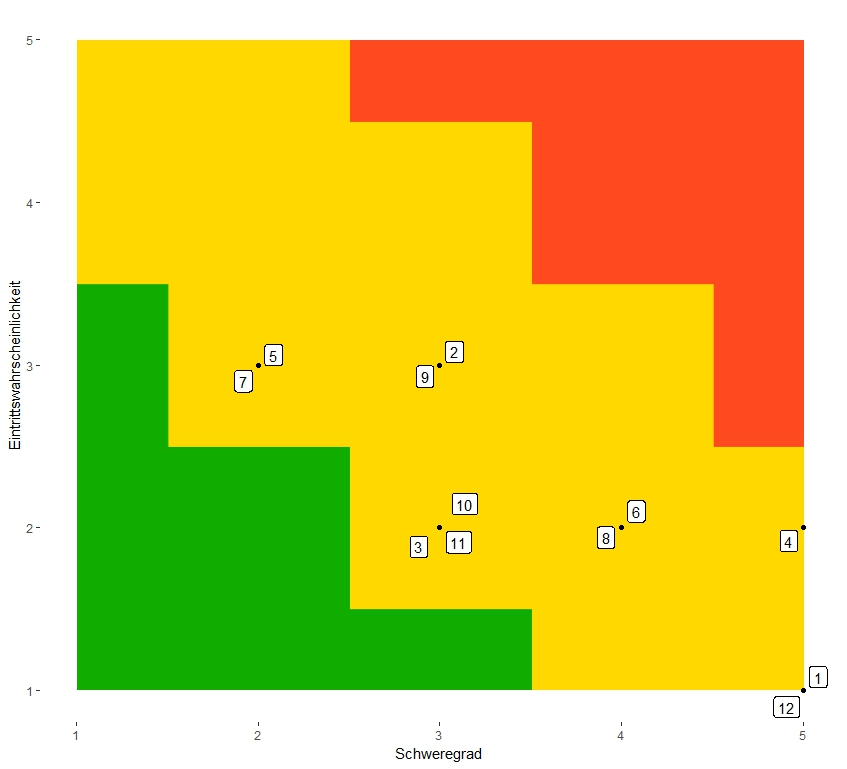
\includegraphics[keepaspectratio,width=\textwidth]{Risikomatrix}
	\end{subfigure}
	\begin{subfigure}[b]{0.45\textwidth}
		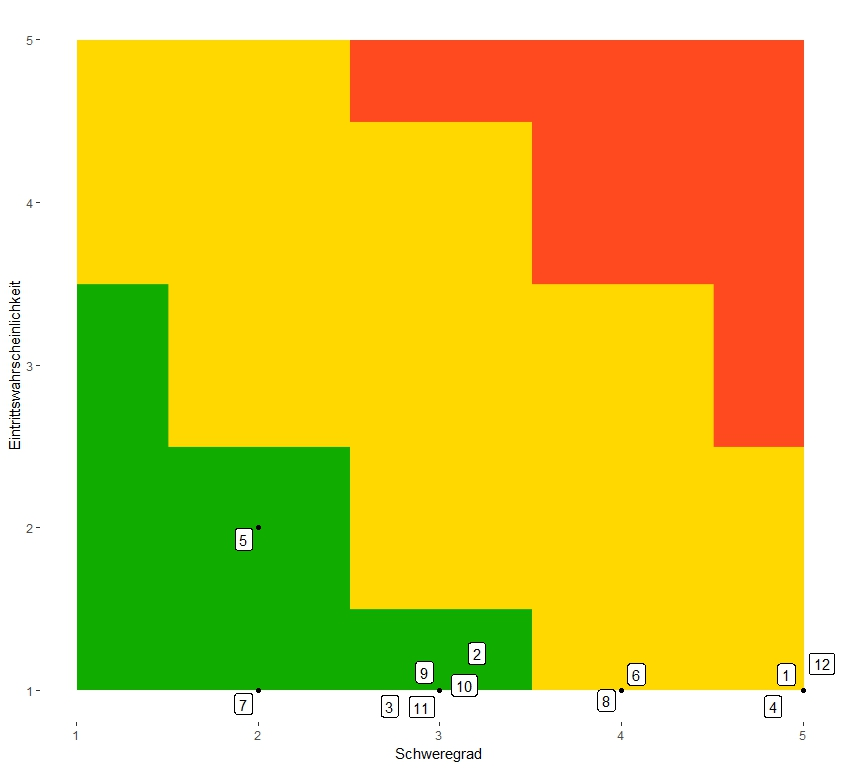
\includegraphics[keepaspectratio,width=\textwidth]{Risikomatrix_nachher}
	\end{subfigure}
	\caption{Gegenüberstellung der Risikomatrizen vor und nach den Massnahmen}
	\label{fig:Gegenueberstellung}
\end{figure}

\begin{figure}[h!]
	\centering
	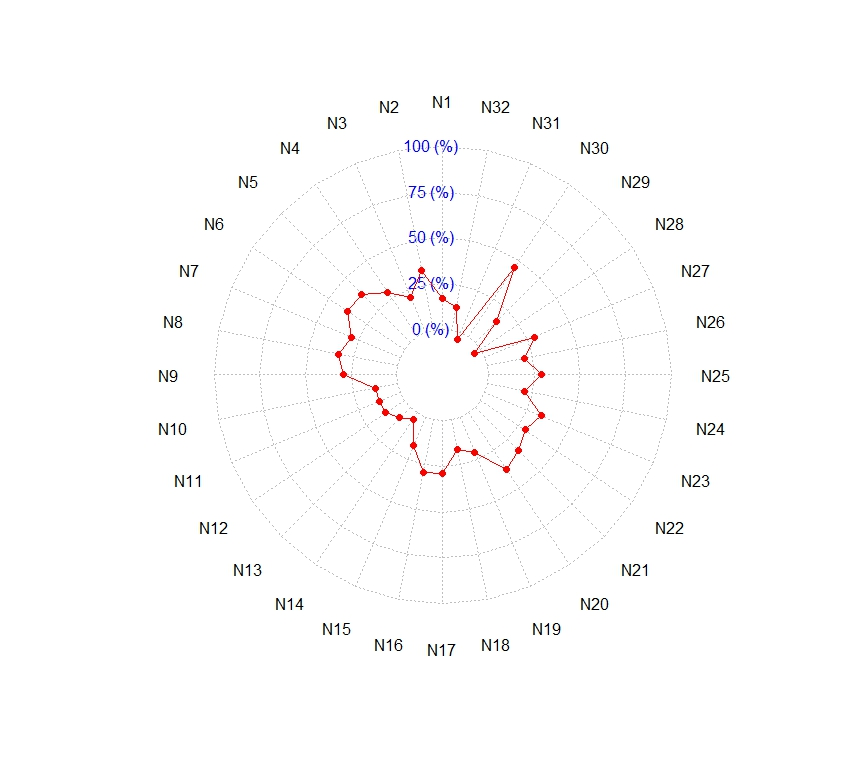
\includegraphics[width=\textwidth,keepaspectratio]{Risikomatrix_Spinne}
	\caption{Die Risiken aus dem Risikokatalog graphisch dargestellt, die rote Linie zeigt die Risiken vor den Massnahmen, während die Grüne die Risiken nach dem Anwenden der Massnahmen darstellt}
	\label{fig:Risikomatrix_Spinne}
\end{figure}

\chapter{Technologierecherche}

Bevor wir mit unserer, eigenständigen Recherche begannen, sassen wir im Team zusammen und machten ein Brainstorming. Dabei kamen wir auf die folgenden Ideen:

\begin{multicols}{2}
\paragraph{Plattformen}
\begin{itemize}[noitemsep]
	\item Rasperry Pi
	\item Arduino
	\item Hifive
\end{itemize}

\paragraph{Programmierprache}
\begin{itemize}[noitemsep]
	\item Python
	\item Java
	\item C\#
	\item Rust
\end{itemize}

\paragraph{Bilderkennung}
\begin{itemize}[noitemsep]
	\item OpenCV
	\item ImageJ
	\item Eigener Algorithmus
\end{itemize}

\paragraph{Position, Last bestimmen \& darstellen}
\begin{itemize}[noitemsep]
	\item 2x 7-Segment
	\item Echolot
	\item Time of Flight
	\item Drehgeber
	\item z-Position
	\item Schrittmotor
	\item LCD
	\item OLED
	\item Bluetooth
\end{itemize}

\paragraph{Zielzone erkennen}
\begin{itemize}[noitemsep]
	\item Kamera
	\item Sensoren
	\item Beleuchtung
\end{itemize}

\paragraph{Startsignal}
\begin{itemize}[noitemsep]
	\item Bluetooth
	\item Knopf
	\item WiFi
	\item Akustisch
\end{itemize}

\paragraph{Energieversorgung}
\begin{itemize}[noitemsep]
	\item Eingebauter Akku
	\item Battery Pack
	\item Li-Ion
	\item NiCad
	\item Supercapacitor (SC)
	\item Bleiakku
	\item Solarpanel
	\item Verbrennungsmotor
	\item Dieselgenerator
	\item Brennstoffzelle
\end{itemize}

\paragraph{Stabilisierung}
\begin{itemize}[noitemsep]
	\item Federn \& Dämpfen
	\item Gyroskop
	\item Tank/Flüssigkeit hin-und herpumpen
	\item Rotoren
	\item Ausgleichsdüsen
\end{itemize}

\paragraph{Antrieb}
\begin{itemize}[noitemsep]
	\item Magnetschwebe
	\item Zeppelin \& Ventilator
	\item Rollen eingeklemmt am Seil
	\item Seilbahn
\end{itemize}

\paragraph{Last anheben/senken}
\begin{itemize}[noitemsep]
	\item Seil
	\item Zahnstange
	\item Teleskoparm
	\item Abwerfen
\end{itemize}
\vspace{2em}
\paragraph{Aufhängung}
\begin{itemize}[noitemsep]
	\item \textquotedblleft Obe druff\textquotedblright
	\item \textquotedblleft Une ane\textquotedblright
	\item Gelenkig \& gedämpft
	\item Heliumballon
\end{itemize}

\paragraph{Last greifen}
\begin{itemize}[noitemsep]
	\item Haken
	\item Saugnapf
	\item Greifer
	\item (Elektro)Magnet
	\item Permanentmagnet
	\item Kranarm
\end{itemize}
\end{multicols}

\subsection{Recherchenbewertung}
Die jeweiligen Quellen werden nach folgendem Schema bewertet:
\begin{itemize}
	\item \textbf{U}mfang (0-5)
	\item \textbf{N}utzen (0-5)
	\item \textbf{B}ewertung = Nutzen + Umfang
\end{itemize}

\vspace{1em}
\noindent
\begin{tabular}{|p{0.3\textwidth}|p{0.02\textwidth}|p{0.02\textwidth}|p{0.02\textwidth}|p{0.5\textwidth}|}
	\hline
	\textbf{Beschreibung} & \textbf{U} & \textbf{N} & \textbf{B} & \textbf{Quelle} \\
	\hline
	Beschreibung der Quelle in Stichworten & 3 & 3 & 6 & [LINK]\\
	\hline
\end{tabular}

\section{Plattformen}
\subsection{Informatik}

\vspace{1em}
\noindent
\begin{tabular}{|p{0.3\textwidth}|p{0.02\textwidth}|p{0.02\textwidth}|p{0.02\textwidth}|p{0.5\textwidth}|}
	\hline
	\textbf{Beschreibung} & \textbf{U} & \textbf{N} & \textbf{B} & \textbf{Quelle} \\
	\hline
	TinkerBoard & 3 & 3 & 6 & https://goo.gl/tBE2uP\\
	\hline
	Raspberry Pi 3 Model B & 1 & 3 & 4 & https://goo.gl/zV2NYF \\
	\hline
	Banana PI M2 Berry & 2 & 3 & 5 & http://www.banana-pi.org/m2ub.html \\
	\hline
	BeagleBone Black Rev & 1 & 2 & 3 & https://beagleboard.org/black/\\
	\hline
	RasPi vs TinkerBoard & 3 & 3 & 6 & https://goo.gl/UeD7um\\
	\hline
	RasPi vs TinkerBoard & 1 & 3 & 4 & https://goo.gl/a3ucY6\\
	\hline
	RasPi vs BananaPi & 2 & 3 & 5 & https://goo.gl/F4eXrp\\
	\hline
	RasPi vs BananaPi & 3 & 5 & 8 & https://goo.gl/JRHX78\\
	\hline
\end{tabular}

\vspace{1em}
Sowohl bei dem Raspberry Pi als auch beim Tinkerboard sind WLAN und Bluetooth
Schnittstellen inbegriffen. Zum benutzen von OpenCV ist eine MMU und eine FPU
notwendig. Deshalb kommen nur Boards in Frage die einen ARM Cortex-A Prozessor
haben. Da aber das TinkerBoard eher dürftige Dokumentation und Unterstützung von Software besitzt \parencite[Fazit]{Finnamore2017} bevorzugen wir das Raspberry Pi.

\subsection{Elektrotechnik}

\subsubsection{Quellen}
\begin{tabular}{|p{0.3\textwidth}|p{0.02\textwidth}|p{0.02\textwidth}|p{0.02\textwidth}|p{0.5\textwidth}|}
	\hline
	\textbf{Beschreibung} & \textbf{U} & \textbf{N} & \textbf{B} & \textbf{Quelle} \\
	\hline
	Hi-/LoFive Kurzbeschreibung & 2 & 2 & 4 & http://alturl.com/b7zyd \\
	\hline
	SiFive Controller Manual \& Cons & 5 & 4 & 9 & http://alturl.com/objsw \\
	\hline
	SiFive Datasheet & 3 & 5  & 8 & http://alturl.com/7t4ya \\
	\hline
	SiFive userlevel ISA & 5 & 3 & 8 & http://alturl.com/9rvz6 \\
	\hline
\end{tabular}

\vspace{1em}
\noindent
\begin{tabular}{|p{0.3\textwidth}|p{0.33\textwidth}|p{0.3\textwidth}|}
  \hline
  \textbf{Name} & \textbf{Vorteile} & \textbf{Nachteile} \\
  \hline
	Arduino Uno R3 & Hoher Verbreitungsgrad, viel bestehende Software & 8-bit MCU \\
	\hline
  Lofive & Hat einen RV32IMAC Prozessor, verwendet einen externen Programmierer, ist die Abgespeckte version vom Hifive Board das besser für die Integration in ein Produkt geeignet ist & Keine \\
  \hline
  Hifive & Hat einen RV32IMAC Prozessor, ist Pin-Kompatibel mit Arduino & Hat die Hardware für die Programmierung auf dem Board \\
  \hline
\end{tabular}
\section{Programmiersprache}


\subsection{Informatik}
Die nachfolgende Recherche wurde unter der Annahme gemacht, dass wir in der Informatik das Raspberry Pi (nachfolgend RasPi genannt) als Plattform benutzen werden. Generell sollte aber Vor- und Nachteile der Sprachen universell sein.

\vspace{1em}
\noindent
\begin{tabular}{|p{0.3\textwidth}|p{0.02\textwidth}|p{0.02\textwidth}|p{0.02\textwidth}|p{0.5\textwidth}|}
	\hline
	\textbf{Beschreibung} & \textbf{U} & \textbf{N} & \textbf{B} & \textbf{Quelle} \\
	\hline
	RasPi untersützte Sprachen & 1 & 4 & 5 & https://goo.gl/WDpi2P \\
	\hline
	Interpreted languages: Pros \& Cons & 1 & 3 & 4 & https://goo.gl/UGrLT5 \\
	\hline
	Python Pro and Cons & 3 & 4  & 7 & https://goo.gl/WURUwZ \\
	\hline
	Python Pro and Cons & 3 & 4 & 7 & https://goo.gl/ci1GbT \\
	\hline
	Python Beginners Guide & 3 & 5 & 8 & https://goo.gl/AqoHsx\\
	\hline
	C Pro and Cons & 3 & 3 & 6 & https://goo.gl/DLEuqR \\
	\hline
	C++ Pro and Cons & 3 & 4 & 7 & https://goo.gl/X4sef2\\
	\hline
\end{tabular}

\subsection{Elektronik}
Da einen Mikrocontroller verwendet wird, welcher für Real-Time Aufgaben
geeignet ist, sind die Optionen relativ limitiert.

\vspace{1em}
\noindent
\begin{tabular}{|p{0.3\textwidth}|p{0.02\textwidth}|p{0.02\textwidth}|p{0.02\textwidth}|p{0.5\textwidth}|}
	\hline
	\textbf{Beschreibung} & \textbf{U} & \textbf{N} & \textbf{B} & \textbf{Quelle} \\
	\hline
  Rust vs C pitfalls & 3 & 3 & 6 & http://www.garin.io/rust-vs-c-pitfalls \\
  \hline
  C++ embedded systems & 3 & 3 & 6 & https://electronics.stackexchange.com/questions/3027/is-c-suitable-for-embedded-systems \\
	\hline
\end{tabular}

\vspace{1em}
\noindent
\begin{tabular}{|p{0.3\textwidth}|p{0.3\textwidth}|p{0.3\textwidth}|}
  \hline
  \textbf{Name} & \textbf{Vorteile} & \textbf{Nachteile} \\
  \hline
  C & Ist Effizient und hat eine hohe Bekanntheit und Verbreitung & Erfordert grosse Kompetenz vom Entwickler zum sicherstellen das keine Sicherheitslücken durch Buffer-Overflows, Undefiniertes-Verhalten durch Compiler Optimierungen oder falsches Verständniss des Memory-Models. \\
  \hline
  C++ & Keine & Weniger Effizient als C wegen Pointer indirection beim Aufruf von Klassenmethoden (dynamic dispatch) und C++ standard library braucht einen Memory Allocator \\
  \hline
  Rust & Gleiche Effizienz wie C oder C++ je nach Programmierstil. Kompiler prüft zur Kompilationszeit das der Code kein Undefiniertes-Verhalten, Memory Errors und Buffer-Overflows hat. Braucht nicht zwingend einen Memory Allocator und unterstützt moderne Programmierkonzepte wie Closures ohne overhead oder Garbage Collector. & Das Rust Ecosystem im Bereich Embedded-Systems ist noch jung, das bedeutet, dass Codesegmente implementiert werden müssen, welche bei anderen Sprachen im Internet verfügbar sind.\\
  \hline
\end{tabular}

\section{Bilderkennung}

\vspace{1em}
\noindent
\begin{tabular}{|p{0.3\textwidth}|p{0.02\textwidth}|p{0.02\textwidth}|p{0.02\textwidth}|p{0.5\textwidth}|}
	\hline
	\textbf{Beschreibung} & \textbf{U} & \textbf{N} & \textbf{B} & \textbf{Quelle} \\
	\hline
	Pi Camera Module & 1 & 2 & 3 & https://www.pi-shop.ch/raspberry-pi-kamera-module-v2\\
	\hline
	Pi Camera With LED & 1 & 2 & 3 & https://www.pi-shop.ch/pi-supply-bright-pi-bright-white-und-ir-kamera-licht-fuer-raspberry-pi\\
	\hline
	Pi Camera und OpenCV mit Python & 4 & 3 & 7 & https://goo.gl/arrQw6 \\
	\hline
	OpenCV & 3 & 3 & 6 & http://opencv.org \\
	\hline
	OpenCV mit Python & 5 & 3 & 8 & OpenCV with Python By Example \\
	\hline
	Bildverarbeitung mit Java (ImageJ) & 5 & 2 & 7 & Digitale Bildverarbeitung - Eine Einführung mit Java und ImageJ\\
	\hline
	ImageJ & 3 & 2 & 5 & https://imagej.net/ImageJ \\
	\hline
	Fiji & 2 & 2 & 4 & http://fiji.sc/ \\
	\hline
	ImageJ Bildprozessierung & 4 & 2 & 6 & Image Processing with ImageJ 2nd Edition \\
	\hline
	Eigener Algorithmus & 5 & 2 & 7 & Computer Vision: Algorithms and Applications\\
	\hline
\end{tabular}

\section{Stabilisierung}

\vspace{1em}
\noindent
\begin{tabular}{|p{0.3\textwidth}|p{0.02\textwidth}|p{0.02\textwidth}|p{0.02\textwidth}|p{0.5\textwidth}|}
	\hline
	\textbf{Beschreibung} & \textbf{U} & \textbf{N} & \textbf{B} & \textbf{Quelle} \\
	\hline
	Federn &4 &4 &8 & Roloff/Mathek Maschinenelemente \\
	\hline
	Dämpfung durch Fluidreibung &3 &3 &6 & Fluidunterricht ThFl 1+2 \\
	\hline
	Gyroskop &2 &1 &3 & https://experimentis-shop.de/gyroskop-in-retroverpackung\_detail\_277.html \\
	\hline
	Gyroskop Physikalische Grundlagen &4 &2 &6 & https://goo.gl/bLthBb \\
	\hline
	Kreiselphänomene &2 &2 &4 & https://goo.gl/Yh2P95 \\
	\hline
	verschiedene Dämpfer &2 &2 &4 & https://goo.gl/zKfMbc \\
	\hline
	Drallsatz: Kreisel und Präzession &3 &2 &5 & Mechanikunterricht Mathphys2 \\
	\hline
	Schwingungen &4 &5 &9 & Physikunterricht Mathphys2 \\
	\hline
	Anfahrregelung &4 &2 &6 & http://www.kran-forum.com/showtopic.php?threadid=1416 \\
	\hline
	Pendelregelung und -Steuerung &4 &1 &5 & vdi norm 4468 eine pendelregelung und- steuereung \\
	\hline
	Elektronische Pendeldämpfung für Krane &2 &1 &3 & https://goo.gl/uN92hp\\
	\hline
\end{tabular}

\section{Masse des Klotzes}
\label{sec:RechKlotzMasse}
Die Masse des Klotzes lässt sich leicht mit der unten Beschriebenen Formel abschätzen.  \\
\begin{displaymath}
	m=V*\rho
\end{displaymath}
$V_{Klotz}=(5cm)^3=125cm^3=125\cdot10^{-6} m^3$ \\
$\rho_{Buche}=690\frac{kg}{m^3}$, $\rho_{Tanne}= 410\frac{kg}{m^3}$ \\
$\Rightarrow$ $m_{Buche} \approx 86.25$g \hspace*{10mm} $m_{Tanne} \approx 51.25$g

\section{Aufhängung}
	\subsection{Rollen}
	\begin{tabular}{|p{0.3\textwidth}|p{0.02\textwidth}|p{0.02\textwidth}|p{0.02\textwidth}|p{0.5\textwidth}|}
		\hline
		\textbf{Beschreibung} & \textbf{U} & \textbf{N} & \textbf{B} & \textbf{Quelle} \\
		\hline
		Rollen &5 &5 &10 & https://www.conrad.ch/de/umlenkrollen-seilrollen-o2304305.html
		\newline https://knupfer.info/shop/index.php \\
		\hline
	\end{tabular}


		Rollen sind auf Modellbauseiten in Praktisch allen grössen erhältlich, falls nötig wäre auch eine kostengünstige Nachbearbeitung möglich.
	\subsection{Federn und Dämpfer}
		\begin{tabular}{|p{0.3\textwidth}|p{0.02\textwidth}|p{0.02\textwidth}|p{0.02\textwidth}|p{0.5\textwidth}|}
		\hline
		\textbf{Beschreibung} & \textbf{U} & \textbf{N} & \textbf{B} & \textbf{Quelle} \\
		\hline
		Dämpfer &3 &3 &6 & https://www.conrad.ch/de/stossdaempfer-o1202411.html \\
		\hline
		Federn &5 &3 &8 & Normteilkatalog\\
		\hline
	\end{tabular}


		Öldruckstossdämpfer sind im Internet für eine Länge von 55-110mm erhältlich. Ihre Dämpflänge liegt zwischen 10-20mm. Bei einigen Modellen kann man die Dämpflänge variieren. \\
		Federn sind als Normteile in praktisch allen möglichen Ausführungen erhältlich. Die kleinsten Durchmesser einer Drehfeder liegt bei ca. 3mm. Das Moment welches übertragen werden kann, liegt bei dieser grösse bei 2.3Nmm

\section{Antrieb}
\begin{tabular}{|p{0.3\textwidth}|p{0.02\textwidth}|p{0.02\textwidth}|p{0.02\textwidth}|p{0.5\textwidth}|}
	\hline
	\textbf{Beschreibung} & \textbf{U} & \textbf{N} & \textbf{B} & \textbf{Quelle} \\
	\hline
	Antrieb DC-Motor & & & & https://www.digikey.ch/product-detail/de/parallax-inc/900-00008/900-00008-ND/1774454 \\
	\hline
\end{tabular}

\section{Antriebsübertragung}
	\subsection{Riemen \& Riemenscheibe}
		\begin{tabular}{|p{0.3\textwidth}|p{0.02\textwidth}|p{0.02\textwidth}|p{0.02\textwidth}|p{0.5\textwidth}|}
		\hline
		\textbf{Beschreibung} & \textbf{U} & \textbf{N} & \textbf{B} & \textbf{Quelle} \\
		\hline
		Riemen &4 &4 &8 & PR+SY
		\newline https://www.conrad.ch/de/antriebsriemen-c32457.html \\
		\hline
		Riemenscheibe &3 &3 &6 &https://www.conrad.ch/de/aluminium-zahnriemenscheibe-reely-bohrungs-o-6-mm \\
		\hline
	\end{tabular}


		Kleine Zahnriemen sind mit einem Umfang von 245-800mm erhältlich. Der kleinste Durchmesser von der passenden Riemenscheibe beträgt 26mm und hat eine Bohrung von \O \,6mm. Die Bohrung kann ohne weiteres auf den Motorflansch angepasst werden.

\section{Positionsbestimmung}

\vspace{1em}
\noindent
\begin{tabular}{|p{0.3\textwidth}|p{0.02\textwidth}|p{0.02\textwidth}|p{0.02\textwidth}|p{0.5\textwidth}|}
	\hline
	\textbf{Beschreibung} & \textbf{U} & \textbf{N} & \textbf{B} & \textbf{Quelle} \\
	\hline
	Sensor Funktionsweise und Physik & 5 & 3 & 8 & Handbook of Modern Sensors \\
	\hline
	Sensorwahl & 5 & 3 & 8 & https://goo.gl/DoJYxL \\
	\hline
	Kalman Filter & 3 & 3 & 6 & https://goo.gl/jj7BRU \\
	\hline
	Multisensor Data Fusion & 5 & 3 & 8 & Multisensor Data Fusion: An Introduction \\
	\hline
	$\text{I}^2\text{C}$ bitbanging & 5 & 5 & 10 & https://goo.gl/Bm3vu8 \\
	\hline
\end{tabular}

\vspace{1em}
\noindent

\subsection{Inertial Measurement Unit}
Eine IMU enthält ein x-y-z Beschleunigungssensor und x-y-z
Gyroskop. Dient zur Unterstützung der Bilderkennung und der Distanz
Messungen. Auch wenn schlussendlich keine IMU benötigt wird ist es trotzdem
ratsam eine zu verbauen, da es schlecht nachträglich hinzugefügt werden kann.

\vspace{1em}
\noindent
\begin{tabular}{|p{0.25\textwidth}|p{0.2\textwidth}|p{0.2\textwidth}|p{0.25\textwidth}|}
  \hline
  \textbf{Name} & \textbf{Interface} & \textbf{Preis} & \textbf{Datenblatt} \\
  \hline
  LSM6DS3US & $\text{I}^2\text{C}$ oder SPI & 3 CHF & https://goo.gl/erby3f \\
  \hline
\end{tabular}

\subsection{Distanz Sensoren}
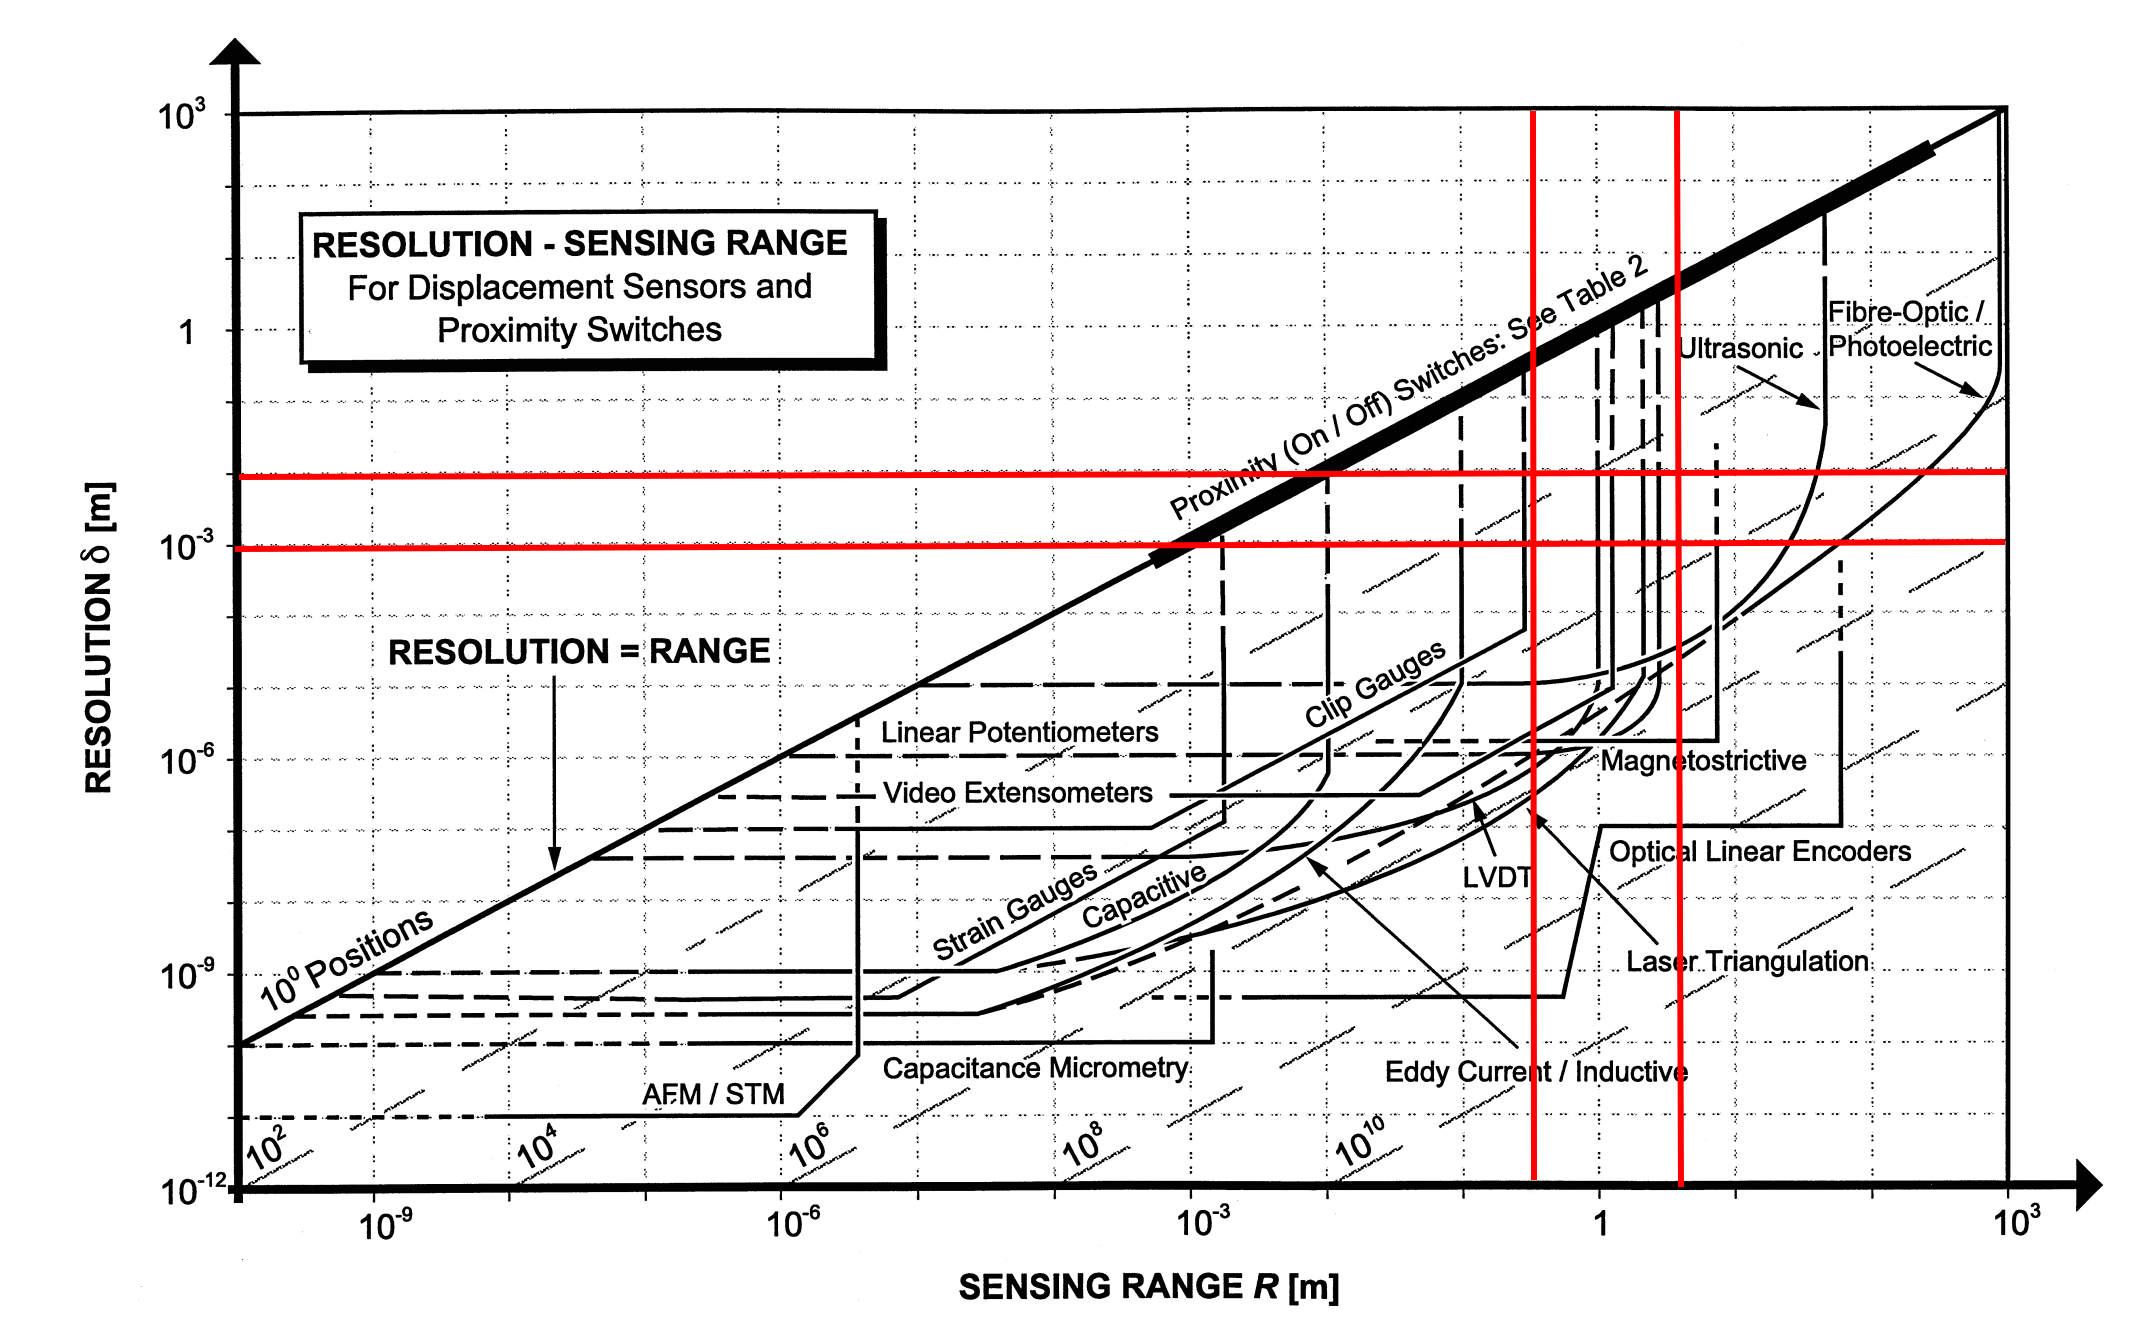
\includegraphics[width=\textwidth]{DistanzSensor}

Daraus schliessen wir das Ultraschall oder Photoelektrische
Sensoren für unsere Anwendung am Besten geeignet sind.

\subsubsection{Distanz Messung in Z-Richtung}
Assistieren der Bilderkennung beim erkennen von Hindernissen und
abschätzen der Z-Höhe des Ladegutes. Je nach dem was für einen Motor gewählt
wird kann dieser zur Abschätzung beitragen wie auch der Beschleunigungssensor
in Z-Richtung. Je nach Grösse der Schwankungen in Y-Richtung kann das Gyroskop
in Y-Richtung auch zur präzise Messung beitragen.

\vspace{1em}
\noindent
\begin{tabular}{|p{0.2\textwidth}|p{0.8\textwidth}|}
  \hline
  \textbf{Anforderung} & \textbf{Grösse} \\
  \hline
  Reichweite & 60cm-110cm \\
  \hline
  Genauigkeit & 1cm \\
  \hline
\end{tabular}

\vspace{1em}
\noindent
\begin{tabular}{|p{0.2\textwidth}|p{0.15\textwidth}|p{0.15\textwidth}|p{0.4\textwidth}|}
  \hline
  \textbf{Name} & \textbf{Interface} & \textbf{Preis} & \textbf{Datenblatt} \\
  \hline
  VCNL4200 & $\text{I}^2\text{C}$ & 3 CHF & https://www.vishay.com/optical-sensors/list/product-84430/ \\
  \hline
\end{tabular}

\subsubsection{Distanz Messung in X-Richtung}
Genaue Positionsbestimmung auf der X-Achse.\\
Mögliche Lösungsansätze (oder Kombination von Lösungsansätze) zu
evaluieren
\begin{itemize}
\item Ultraschall oder Photoelektrische Sensoren, obwohl aufgrund der Zeichnung
  das fehlen einer schönen Fläche vorne oder hinten zum Problem werden könnte.
\item Positionsbestimmung durch messen abgefahrener Strecke
\item Positionsbestimmung durch messen der Beschleunigung in X-Richtung
\item Positionsbestimmung durch Feature-Tracking
\end{itemize}

\section{Positionsanzeige}
\vspace{1em}
\noindent
\begin{tabular}{|p{0.3\textwidth}|p{0.02\textwidth}|p{0.02\textwidth}|p{0.02\textwidth}|p{0.5\textwidth}|}
	\hline
	\textbf{Beschreibung} & \textbf{U} & \textbf{N} & \textbf{B} & \textbf{Quelle} \\
	\hline
	LCD Modul & 1 & 3 & 4 & https://www.sparkfun.com/products/9394 \\
	\hline
	RPI Bluetooth & 2 & 3 & 5 & https://github.com/EnableTech/raspberry-bluetooth-demo \\
	\hline
\end{tabular}

\section{Energieversorgung}
\vspace{1em}
\noindent
\begin{tabular}{|p{0.3\textwidth}|p{0.02\textwidth}|p{0.02\textwidth}|p{0.02\textwidth}|p{0.5\textwidth}|}
	\hline
	\textbf{Beschreibung} & \textbf{U} & \textbf{N} & \textbf{B} & \textbf{Quelle} \\
	\hline
	LiPo & 1 & 3 & 4 & https://hobbyking.com/en\_us/lipo.html \\
	\hline
	Ladegerät & 1 & 3 & 4 & https://hobbyking.com/en\_us/imax-b6ac-v2-professional-balance-charger-discharger.html \\
	\hline
	Batterie-Packet & 1 & 1 & 2 & https://www.conrad.ch/de/batteriehalter-4x-mignon-
	aa-kabel-l-x-b-x-h-63-x-55-x-16-mm-mpd-ba4aaw-1555
	538.html?sc.ref=Search\%20Results
	\\
	\hline
\end{tabular}

\section{Last anheben/senken}
\begin{tabular}{|p{0.3\textwidth}|p{0.02\textwidth}|p{0.02\textwidth}|p{0.02\textwidth}|p{0.5\textwidth}|}
	\hline
	\textbf{Beschreibung} & \textbf{U} & \textbf{N} & \textbf{B} & \textbf{Quelle} \\
	\hline
	Antriebsmotor, 12VDC, 3W, 0.05Nm & & & &
	http://ch.farnell.com/airpax/9904-120-52602/getriebemotor-12v-dc-330-u-min/dp/147874  \\
	\hline
	div. Typen & & & & http://www.directindustry.de/prod/johnson-electric/product-665-470175.html\\
	\hline
	12VDC, \textbf{85rpm}, 2~3W & & & & https://goo.gl/NfN4xx\\
	\hline
	Gleitlager, 3mm & & & & http://www.cncshop.at/index.php?k=165\\
	\hline
\end{tabular}

\section{Startsignal}
\subsection{Mechanisch – Knopf}
Keine Datenübertragung, Einfach, keine Parameter

\subsection{Bluetooth}
Datenübertragung, direkt Sicht nötig, Parameter möglich, Geringer Energiebedarf, aufwendiges Pairing.
Kann gleichzeitig verwendet werden um während des Entwicklungs- und Test-Prozesses Daten (v.a. Software-Updates) an die Laufkatze zu senden. Zudem könnten während Entwicklung und Betrieb Daten an eine Auswertungseinheit (Debugging) (z.B. Laptop oder anderes Mobilgerät) gesendet werden.

\subsection{WiFi}
Datenübertragung, weite Distanzen möglich, Userinterface einfach zu bauen, Parameterübergabe möglich, Verbinden dauert unter Umständen lange, Ad-hoc Verbindungen
Kann gleichzeitig verwendet werden um während des Entwicklungs- und Test-Prozesses Daten (v.a. Software-Updates) an die Laufkatze zu senden. Zudem könnten während Entwicklung und Betrieb Daten an eine Auswertungseinheit (Debugging) (z.B. Laptop oder anderes Mobilgerät) gesendet werden.

\subsection{Akustisch}
Mikro nötig, Falscherkennung Signal als Risiko, zusätzliche Bibliotheken welche sonst nicht benötigt werden.

\subsection{Licht}
Einfach, Problem Abschirmung \& Fremdsignale.

\vspace{1em}
\noindent
\begin{tabular}{|p{0.3\textwidth}|p{0.02\textwidth}|p{0.02\textwidth}|p{0.02\textwidth}|p{0.5\textwidth}|}
	\hline
	\textbf{Beschreibung} & \textbf{U} & \textbf{N} & \textbf{B} & \textbf{Quelle} \\
	\hline
	Lichtsensor bauen & 2 & 1 & 3 & http://www.instructables.com/id/Highly-sensitive-Arduino-light-sensor/ \\
	\hline
\end{tabular}


\section{Endschalter}
\begin{tabular}{|p{0.3\textwidth}|p{0.02\textwidth}|p{0.02\textwidth}|p{0.02\textwidth}|p{0.5\textwidth}|}
	\hline
	\textbf{Beschreibung} & \textbf{U} & \textbf{N} & \textbf{B} & \textbf{Quelle} \\
	\hline
	Endschalter Hebelarm & 1 & 2 & 3 & https://goo.gl/W2no2b\\
	\hline
	Hebelarm & 1 & 2 & 3 & http://www.robotshop.com/ca/en/micro-contact-limit-switch.html\\
	\hline
\end{tabular}

\section{Last greifen}
\begin{tabular}{|p{0.3\textwidth}|p{0.02\textwidth}|p{0.02\textwidth}|p{0.02\textwidth}|p{0.5\textwidth}|}
	\hline
	\textbf{Beschreibung} & \textbf{U} & \textbf{N} & \textbf{B} & \textbf{Quelle} \\
	\hline
	Greifer, Krangreifer &4 &2 &6 & https://goo.gl/TCDBLD \\
	\hline
	Greifer, Greifer Festo &3 &1 &4 & https://goo.gl/4LkLtu\\
	\hline
	Greifer Festo 2 &4 &3 &7 & https://goo.gl/ZBjYKg\\
	\hline
	Zylinder Elektronisch, Phoenix Mecano &3 &3 &6 & https://goo.gl/zbZbAp\\
	\hline
	Elektromagnet maqna &3 &4 &7 & https://goo.gl/RpFgQZ\\
	\hline
	Goudsmit Elektro-magneten &3 &2 &5 & https://goo.gl/FHBsJE\\
	\hline
	Elektromagnet Auslegung &4 &4 &8 & https://goo.gl/H2XLqz\\
	\hline
	Elektro-permanent-magnet - Analytische und Experimentelle Methodologie und Konstruktion & 5 & 3 & 8 & https://goo.gl/29kkM8\\
  \hline
\end{tabular}

\chapter{Grobkonzept / Evaluation Prinzipien}

\section{Mechanik}

\subsection{Morphologischer Kasten Mechanische Komponenten}
% TODO Basil: angepasster Kasten, oder iO, oder entfernen?
\begin{figure}[h!]
	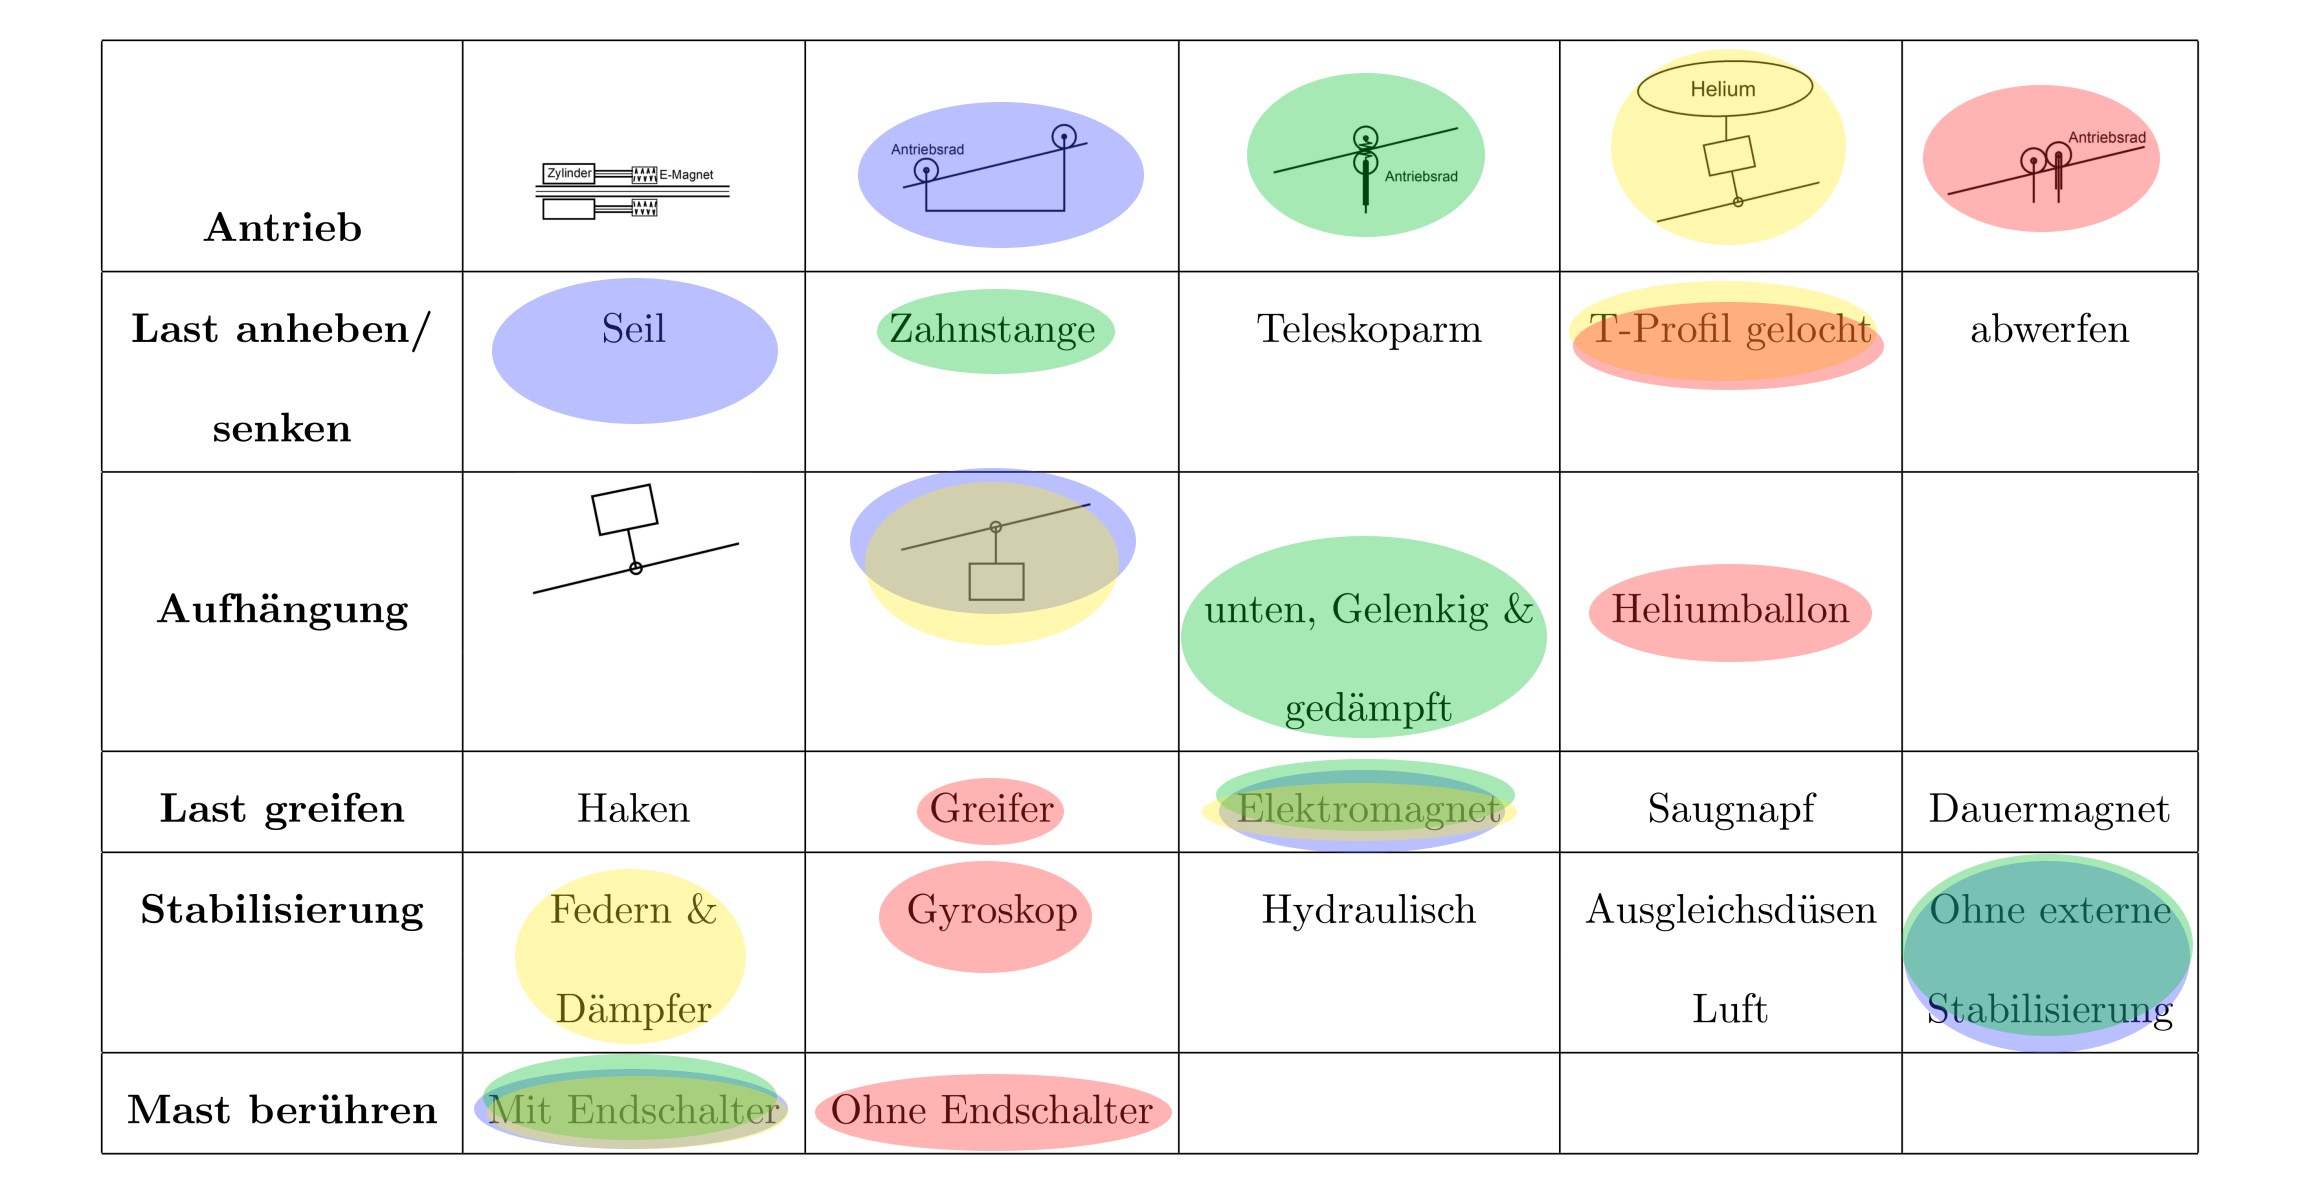
\includegraphics[keepaspectratio,width=\textwidth]{MorphKasten}
	\caption{Mögliche Kombinationen der Komponenten}
	\label{fig:Morphkasten}
\end{figure}
\clearpage

\subsection{Evaluation Antrieb Variante 1}


\subsection{Evaluation Antrieb Variante 2}


\subsection{Evaluation Antrieb Variante 3}


\subsection{Evaluation Lastaufnahme per Seilwinde}


\subsection{Evaluation Lastaufnahme per Zahnstange}


\subsection{Evaluation Aufhängung aufgehängt}


\subsection{Evaluation Aufhängung gedämpft}


\subsection{Evaluation Last per Haacken greifen}


\subsection{Evaluation Last per Dauermagnet greifen}


\subsection{Evaluation Positionsbestimmung per Schrittmotor}


\subsection{Evaluation Positionsbestimmung per Durchhang}



\section{Elektronik}
\subsection{Blockdiagramm}
\begin{figure}[h!]
  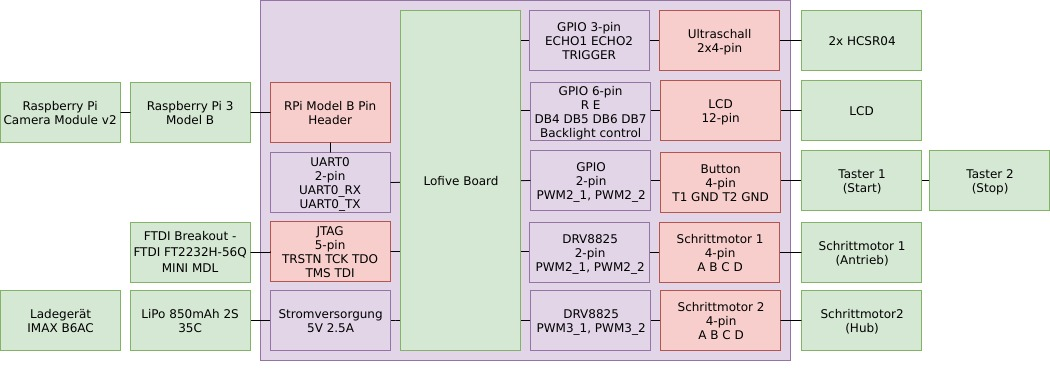
\includegraphics[keepaspectratio,width=\textwidth]{BlockdiagrammElektronik}
  \caption{Blockdiagramm}
  \label{fig:ElektronikBlockdiagramm}
\end{figure}
\newpage
\subsection{Evaluation Elektromagnet}
\subsubsection{Messprotokoll Modell Eigenbau V1.0}
Zur evaluation des Elektromagneten wird ein erstes Modell erstellt, welches aus einer eisenhaltigen Schraube und einer Kupferwicklung besteht.
\begin{figure}[h!]
	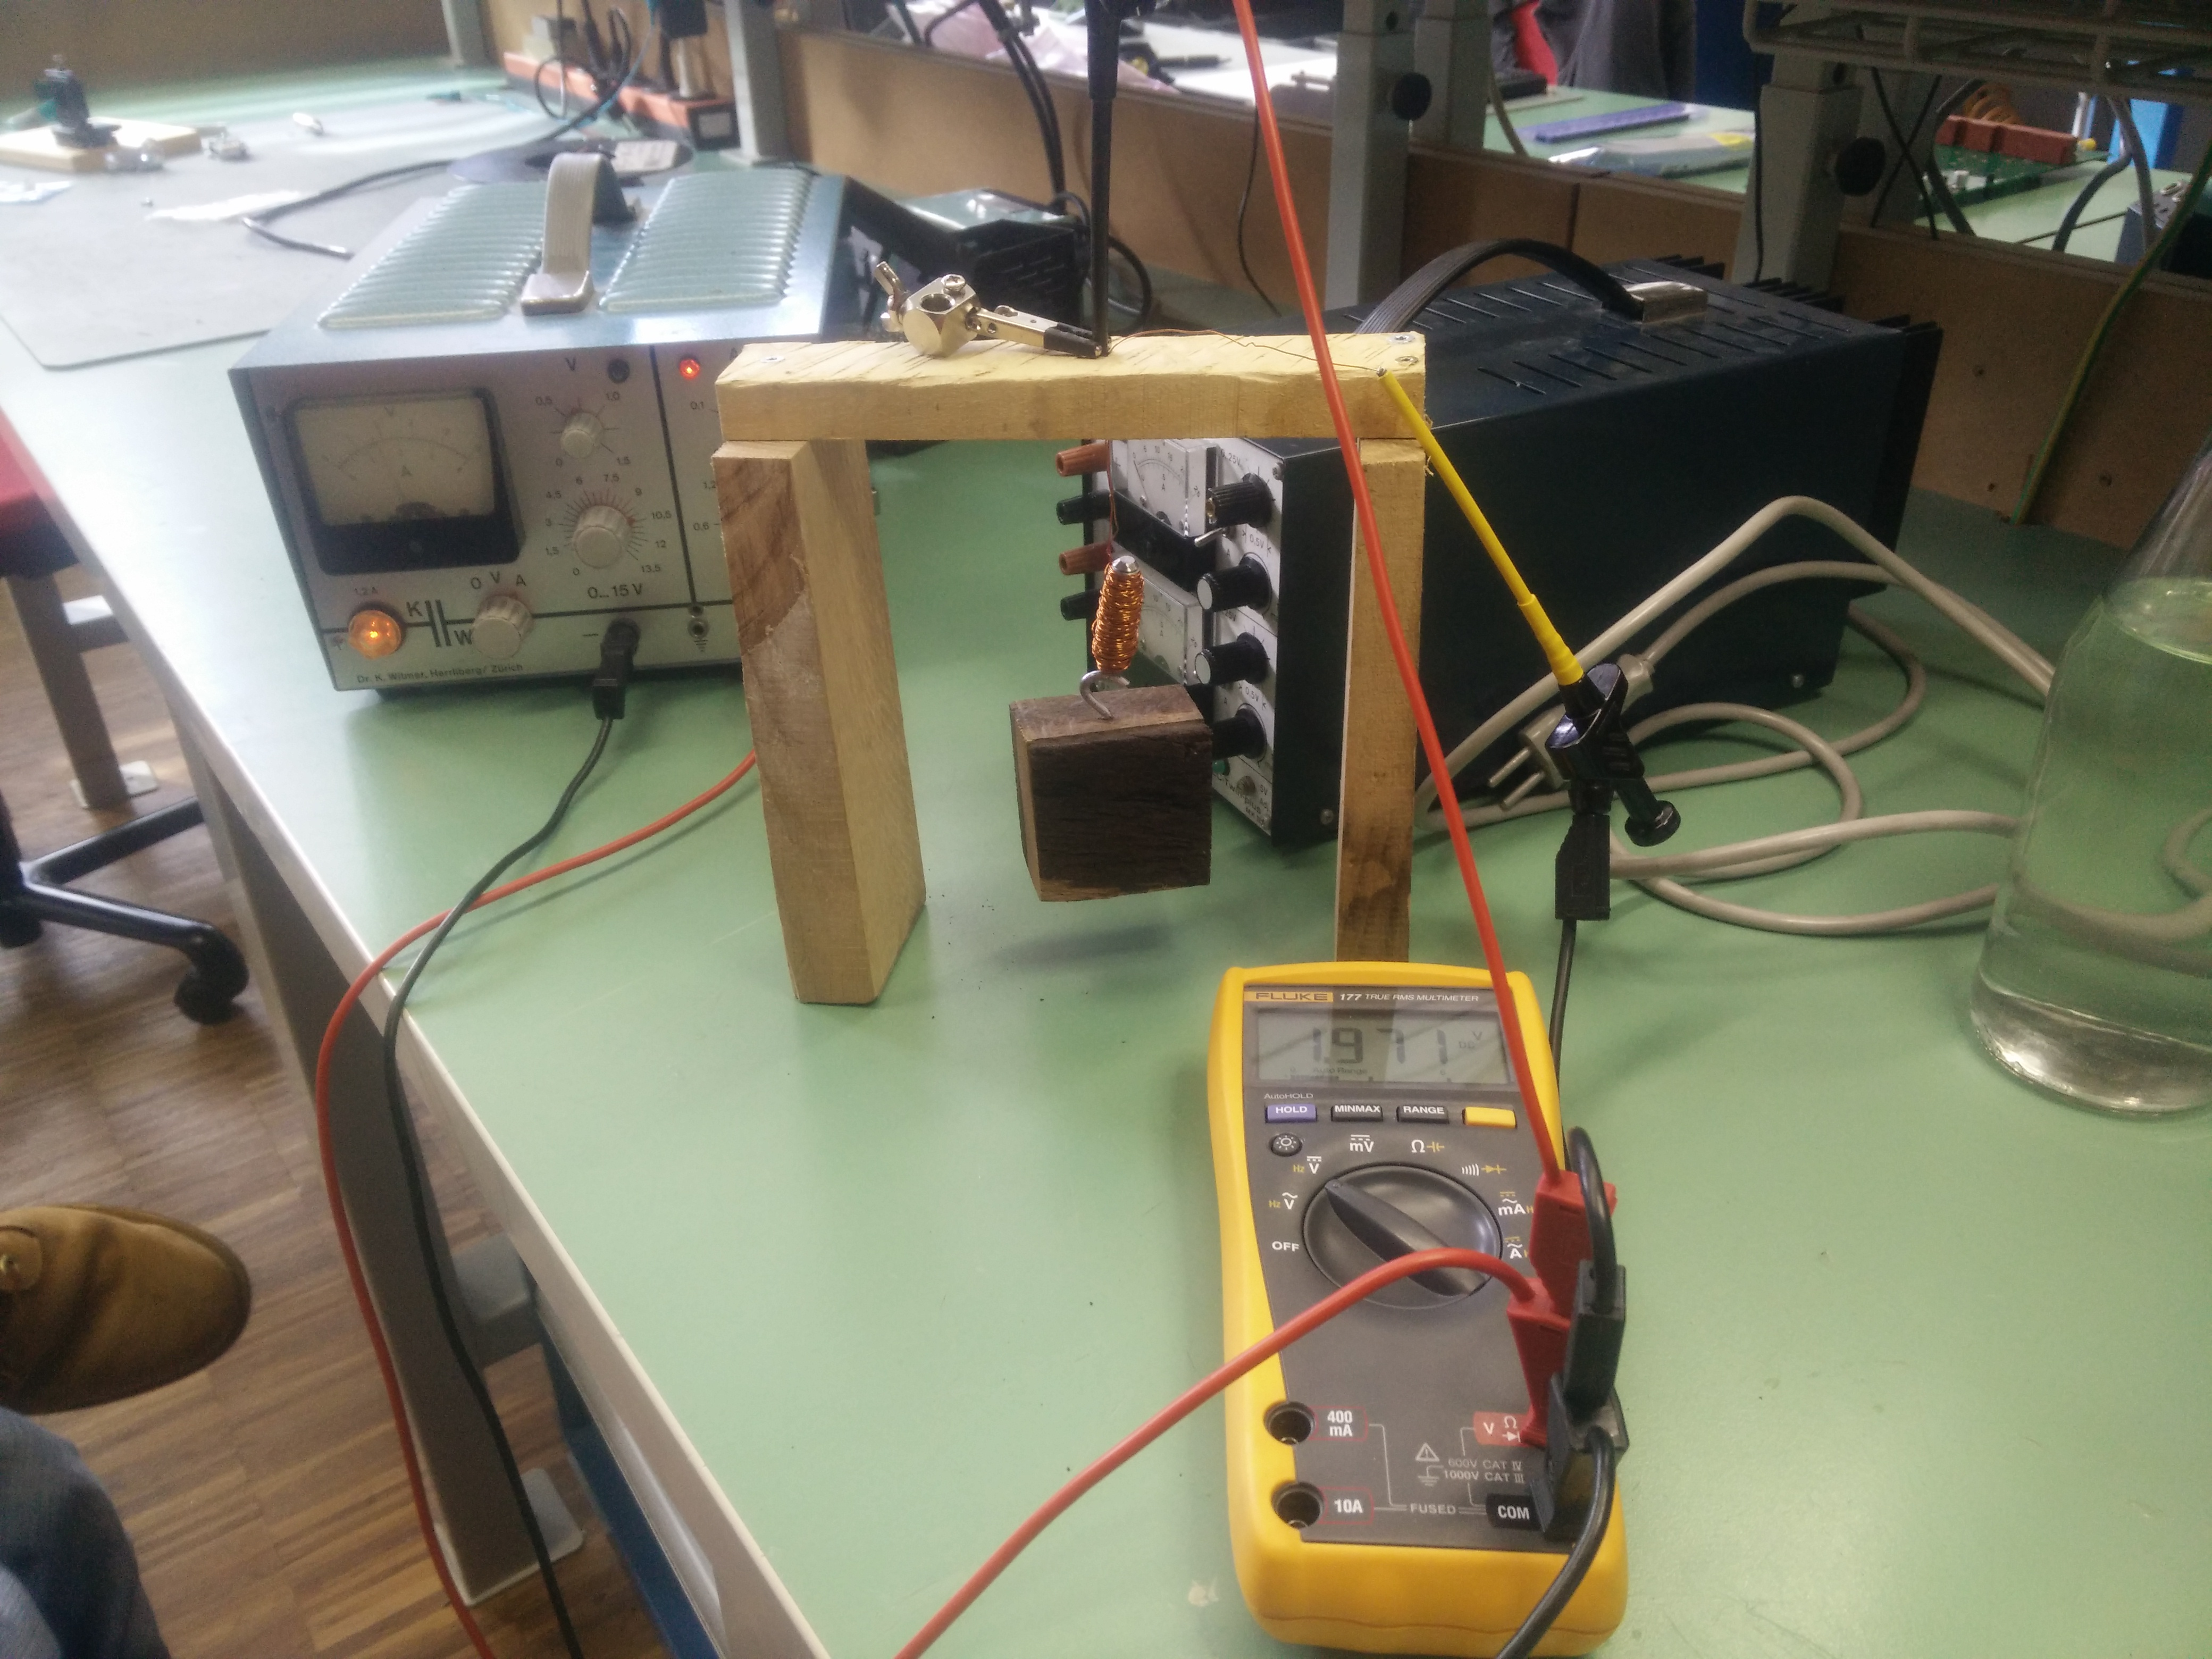
\includegraphics[keepaspectratio,width=\textwidth]{Versuchsaufbau_Elektromagnet_v1}
	\caption{Versuchsaufbau Elektromagnet V1}
	\label{fig:VersuchsaufbauElektromagnet}
\end{figure}

Dabei zeigt sich, dass ein Elektromagnet durchaus zum Heben der vorgegebenen Last in Frage kommt. Jedoch stellt das erste Modell viel mehr ein Heizkörper, als ein ideales Elektromagnet dar.
Daher wird die Entscheidung gefällt eine zweite Version zu erstellen, welche mehr Eisenfläche, eine grössere Wicklungszahl, einen dünneren Draht und dadurch einen geringeren Stromverbrauch aufweist.

\subsection{Elektronik Kosten, Dimensionen und Gewicht}
TODO: Wichtig für Budgetplanung und Machinenbauer

\subsection{Evaluation Lofive Board}
TODO: David Craven
Kritische Sachen die Funktionieren müssen im PREN1. Sonst müssen wir ein anderes
Board verwenden.
Toolchain, Real-Time OS, $\text{I}^2\text{C}$ bitbanging

\subsection{Evaluation Arduino}
TODO Kurzevaluation Arduino (Gewicht, Dimension, Schnittstellen)

\subsection{Energie und Stromversorgung}
TODO: Kritisch für Roboter

\section{Informatik}
Da wir in den verschiedenen Disziplinen unterschiedliche Anforderungen besitzen, trennen wir für die Beschlussfassung diese und bewerten die Teilfunktionen separat.

\subsection{Evaluation Plattformen und Programmiersprachen}
% TODO Stub vergrössern?

Das Rasperry PI ist ein Einplatinencomputer in der Grösse einer
Kreditkarte. Das Ein-Chip-System von Broadcom läuft mit einem ARM-Mikroprozessor.
Durch seine Bekanntheit, der vielen Module die es dazu fertig gibt, sowie seinem Preis ist das Rasperry PI Pionier auf dem Bereich der Einplatinencomputer.

TODO: Detaillierte SPECS Raspi 
https://www.raspberrypi.org/products/raspberry-pi-3-model-b/ 

Die Konkurrenten des Raspberry Pi sind meistens leistungsstärker, dadurch aber auch teurer. Was beim Raspberry Pi immer wieder betont wird, ist die riesige Community und deren Unterstützung. Man kann mit hoher Wahrscheinlichkeit davon ausgehen, dass Teilprobleme, welche wir in diesem Projekt haben werden, bereits von Anderen teilweise oder ganz gelöst und dokumentiert wurden.

Diese Unterstützung einer grossen Community und unsere eigene Unzulänglichkeiten betrachtend, haben wir uns für das Raspberry Pi entschieden.

\begin{tabular}{|l|l|}
	\hline 
	\textbf{Vorteile} & \textbf{Nachteile} \\ 
	\hline 
	+ OS Installation möglich & - Ausführung von Befehlen langsamer  \\ 
	+ Erweiterbarkeit & als bei einfachem Mikrocontroller\\
	+ Unterstützt diverse Programmiersprachen & \\
	+ Einfache Umsetzung bei komplexen Aufgaben & \\
	+ Hoher Bekanntheitsgrad & \\
	+ Grosse Community & \\
	+ Niedriger Preis & \\
	\hline 
\end{tabular} 

Python ist eine objektorientiere Programmiersprache, welche den Ruf hat, sehr
einfach zu erlernen zu sein. Python wird  zur Laufzeit in Maschinensprache
übersetzt. Die Grenzen liegen auf der systemnahen Programmierung (z.B. bei
Gerätetreibern oder optimalen Geschwindigkeiten).

Immer auch unsere eigenen Erfahrungen und Vorkenntnisse im Kopf behaltend, haben wir uns im Informatikerteam entscheiden mit Python zu beginnen. 

\begin{tabular}{|l|l|}
	\hline 
	\textbf{Vorteile} & \textbf{Nachteile} \\ 
	\hline 
	+ Objektorientiert &  Geschwindigkeit im vgl. zu C\\
	+ Einfach zu lernen & \\
	+ Umfangreiche Bibliothek & \\
	+ Kostenlos erhältlich & \\
	\hline 
\end{tabular} 

Die Nachteile von Python liegen vor allem in der Geschwindigkeit der Interpretation, da Python im Vergleich zu C eine interpretierte und keine vorkompilierte Sprache ist. Wir behalten uns vor, den erarbeiteten Code zu C/C++ zu portieren, sollte Geschwindigkeit ein Problem werden.

Bei der Programmiersprache C werden einzelne Anweisungen als Folge
zusammengestellt, welche nacheinander ausgeführt werden. C ist sehr
maschinennah, weshalb sie auch als sehr schnell gilt.

\begin{tabular}{|l|l|}
	\hline 
	\textbf{Vorteile} & \textbf{Nachteile} \\  
	\hline 
	+ Systemnah & - Komplex \\
	+ Geschwindigkeit & \\ 
	\hline 
\end{tabular} 


\subsection{Evaluation Kommunikation zwischen Elektronikkomponenten}

Zwischen dem RaspberryPi und dem Elektronikerboard soll der Informationsaustausch über eine serielle Schnittstelle erfolgen. Entweder über USB oder über die dedizierten Pins asynchron (UART).

\subsubsection{UART}

Für die Verwendung einer Kommunikation mit einer asynchronen, seriellen UART-Schnittstelle können jeweilige PINs verwendet werden. 

Auf dem RaspberryPi können Pin 8 (Tx) und Pin 10 (Rx) verwendet werden.
TODO: BILD: raspberry\_pi3\_model\_b\_pin\_diagram.jpg

Auf Seiten Elektrotechnik TODO. 

Die Pins können für Testzwecke direkt via Kabel miteinander verbunden werden. Im Endausbau soll diese Verbindung jedoch über einen eigenes angefertigten Print laufen. So wird auch sichergestellt, dass beide Boards einen gemeinsamen GROUND haben. 

UART muss auf dem RasperryPi manuell aktiviert werden.  Zusätzlich muss das integrierte Bluetooth-Modul deaktiviert werden, sodass die genannten Ports nicht "miniUART" verwenden. 

Für die serielle Übertragung müssen Baudrate, Port, Databits, Parity Check, Stopbits und flow control sowie ein genaues Nachrichtenformat definiert werden. 

\subsubsection{USB}


\subsection{Evaluation Zielerkennung per Bilderkennung}

Zur Bilderfassung wird eine RaspberryPi Camera v2 verwendet. Das Camera Modul v2 ist 25 x 24 x 9 mm, wiegt ca. 3g und kostet ca. 44 CHF. 
Sie hat einen Sony IMX219 8-megapixel sensor. Die Kamera wird über das CSI-Schnittstelle angeschlossen und gesteuert. Sie ist für Anfänger geeignet, biete jedoch trotzdem viele Funktionen für Fortgeschrittene Nutzer. 
Bereits während der Technologierecherche tauchten viele nützliche Anleitungen auf, in welchen das Camera Module v2 genutzt wurde. 
Zur Ansteuerung mit Hilfe der Programmiersprache Python gibt es eine entsprechende Python-Bibliothek: Picamera. 

\begin{tabular}{|l|l|}
	\hline 
	\textbf{Vorteile} & \textbf{Nachteile} \\  
	\hline 
	+ Einfach zu verbauen &  - Hoher Preis im Vergleich\\
	+ Einfach zu steuern mit Python & \\
	+ kleine Bauform & \\
	+ grosse Community & \\ 
	\hline 
\end{tabular} 

Die Verwendung einer kostengünstigeren USB-Kamera wird ausgeschlossen. 

\begin{tabular}{|l|l|}
	\hline 
	\textbf{Vorteile} & \textbf{Nachteile} \\  
	\hline 
	+ Günstig &  - Grosse Bauform\\
	 & - Treiber nötig \\
	 & - Gewicht \\
	 & - kleine bis keine Community\\ 
	\hline 
\end{tabular} 

TODO Warum OpenCV? 

\subsection{Evaluation Zielerkennung per Infrarotsensor}

Nebst der klassischen Bilderkennung wurde auch eine Variante gesucht, welche ohne Kamera funktionieren könnte. 

Wie erkennt man dunkel/hell?
http://diwo.bq.com/en/black-or-white-the-infrared-sensor/

Sensor und RaspberryPi: 
https://circuitdigest.com/microcontroller-projects/raspberry-pi-ir-sensor-tutorial


\chapter{Lösungskonzeption}
\section{Durchhang}
Der Durchhang des Seils ist abhängig vom Gewicht der Laufkatze. Dabei ist es wichtig den Durchhang für das sichere Überfahren der Hindernisse zu kennen. Zudem besteht die Möglichkeit, die Positionsanzeige in vertikaler Richtung als Funktion der zurückgelegten Strecke abzubilden, womit ein zusätzliches Messsystem weggelassen werden kann.

\subsection{Grobversuch Durchhang}
Es wurde ein einfacher Versuch über den Durchhang des Tragseiles gemacht. Die Dimensionen und Proportionen sind nicht massstäblich, nur Beispielhaft. Dabei wurde ein Seil zwischen zwei Stühlen durch ein Gewicht gespannt. Ein angebrachtes Gewicht wurde dannach an verschiedenen Positionen angehängt und der Durchhang wurde gemessen. Dabei kam raus, dass der maximale Durchhang in der Mitte des Tragseils ist. Der Durchhang im oberen fünftel des Tragseils betrug dabei ungefähr 2/3 des maximalen Durchhangs.
Für eine genaue Funktion des Durchhangs könnten am Musteraufbau Gewichte an verschiedenen Positionen angehängt und der Durchhang von Hand messen. Durch Eingabe in Excel kann somit die Funktion für verschiedene Gewichte ermittelt werden.

\subsection{Rechnung Durchhang}
Die Grundsteigung des Tragseils beträgt 8,2 Grad. Mithilfe von Trigonometrie und der Spannung des Seils konnte der Durchhang in der Mitte des Tragseils näherungsweise ausgerechnet werden.

\vspace{1em}
\noindent
\begin{table}[h!]
	\begin{tabular}{|p{0.15\textwidth}|p{0.2\textwidth}|p{0.55\textwidth}|}
		\hline
		\textbf{Gewicht [kg]} & \textbf{Steigungswinkel [\SI{}{\degree}](ohne Grundsteigung)} &\textbf{Durchhang [cm]}\\
		\hline
		0.5&0,95&2.29\\
		\hline
		1&1,91&5,84\\
		\hline
		1.5&2,87&8,76\\
		\hline
		2&3,82&11,69\\
		\hline
		2.5&4,78&14,63\\
		\hline
		3&5,74&17,59\\
		\hline
		3.5&6,70&20,56\\
		\hline
		4&7,66&23,54\\
		\hline
		4.5&8,63&26,55\\
		\hline
		5&9,59&29,58\\
		\hline
	\end{tabular}

	\caption{Rechnung Durchhang}
	\label{tbl:DurchhangRechnung}
\end{table}

\subsection{Versuch Durchhang}
Durch Anhängen eines Gewichtes in regelmässigen Abständen und über die ganze Strecke verteilt, wurde der jeweilige Durchhang gemessen und danach in einer Excel-Tabelle eingetragen. Durch Erstellen einer Grafik konnte für die Kurve eine Trendlinie erstellt werden. Aus dieser konnte eine Funktion des Durchhanges in Abhängigkeit der Strecke abgeleitet werden. Mit dieser Funktion (siehe Bild \ref{fig:Durchhang_v1}) kann später auch die Position ermittelt werden.
\begin{figure}[h!]
	\centering
	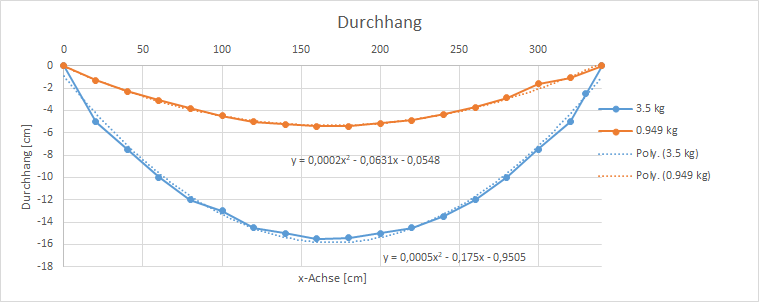
\includegraphics[width=\textwidth,keepaspectratio]{Durchhang_v1}
	\caption{Diagramm zum Durchhang}
	\label{fig:Durchhang_v1}
\end{figure}

Interessant ist, dass die tatsächlichen Werte des Durchhanges schlecht mit den errechneten Werten in Tabelle \ref{tbl:DurchhangRechnung} übereinstimmten. Dies führt daher, dass die Umlenkrollen der Plattform eine grosse Reibung aufweisen und daher die Rechnung mit konstanter Seilspannung eigentlich nicht ganz richtig ist. Die Rollen werden, jedoch von der Modulleitung noch durch Reibungsärmere ersetzt. Danach muss die Durchhangsmessung nochmals durchgeführt werden.

\chapter{Schlussdiskussion}

\chapter*{Verzeichnisse}

\listoffigures

\listoftables
% TODO Tabellen mit Captions versehen

\printbibliography

\appendix

\chapter{Meilensteinberichte}

\chapter{Task-Listen}

\end{document}